\documentclass{mipt-thesis-ms}
% Следующие две строки нужны только для biblatex. Для inline-библиографии их следует убрать.
\usepackage{mipt-thesis-biblatex}
\usepackage{biblatex}
\addbibresource{Diplom.bib}
\usepackage{hyperref}
\usepackage{graphicx}
\usepackage{makecell}
\DeclareGraphicsExtensions{.pdf,.png,.jpg}

\title{Одновременное картирование и локализация по видео с построением плотной карты в реальном времени}
\author{Муравьев К.\,Ф.}
%\supervisor{Яковлев К.\,С.}
%\groupnum{М05-914Б}
%\faculty{Физтех-школа прикладной математики и информатики}
%\department{Кафедра анализа данных}

\begin{document}
	%\frontmatter
	%\maketitle
	\titlecontents
	%\mainmatter
	
	%----------------------------------------------------------------------------------------------------------------------------
	% INTRODUCTION
	%----------------------------------------------------------------------------------------------------------------------------
	
	\chapter{Введение}
	
	В последнее время мобильные роботы и беспилотные летательные аппараты все чаще используются в различных коммерческих и бытовых целях. В некоторых случаях, например, на больших расстояниях или в условиях сильных радиопомех, дистанционное управление подобными аппаратами может быть затруднено. В таких случаях возникает необходимость автономного функционирования беспилотных аппаратов. Для успешного выполнения многих задач в автономном режиме необходимо определять положение аппаратов в пространстве, а также положение окружающих объектов. Возникает задача одновременного картирования и локализации (simultaneous localization and mapping, SLAM).
	
	Решение задачи SLAM зачастую осложняется различными ограничениями. Например, внутри помещений невозможна навигация с помощью GPS; также на малогабаритных роботах ограничения по весу и энергопотреблению не позволяют установить большое количество высокоточных датчиков. В некоторых случаях единственным доступным сенсором является видеокамера. Возникает задача одновременного картирования и локализации по видеопотоку (vision-based SLAM, vSLAM).
	
	Классические методы vSLAM, основанные на извлечении особых точек из изображений \cite{mur2015orb}\cite{klein2007parallel}, имеют существенные недостатки, такие, как необходимость задания масштаба пользователем, потеря локализации при повороте на месте и разреженность построенной карты. Разреженные карты, построенные подобными методами, не пригодны для планирования маршрутов, поскольку маршрут может быть проложен через не нанесенную на карту точку препятствия.
	
	Восстановление карт глубин по видеопотоку позволяет устранить вышеописанные недостатки, сведя задачу vSLAM к задаче одновременного картирования и локализации с использованием видеоданных и данных о глубине (RGBD-SLAM). Для решения задачи RGBD-SLAM разработаны эффективные методы решения с построением плотной карты, например, \cite{endres20133}\cite{labbe2019rtab}.
	
	Для восстановления глубины по видеоданным обычно используются методы, основанные на вычислении оптического потока между соседними кадрами видеоряда. Как правило, производительность таких методов недостаточна для обработки видеопотока в реальном времени с помощью бортовых вычислителей робототехнических систем. Например, обработка одной пары изображений с помощью метода, предложенного в работе \cite{ummenhofer2017demon}, занимает 110 мс на видеокарте GTX Titan. На бортовых компьютерах малогабаритных роботов обработка изображений будет выполняться еще дольше.
	
	В настоящее время помимо классических алгоритмов восстановления глубины применяются также нейросетевые методы, обрабатывающие отдельно каждый кадр видеопоследовательности. Подобные методы позволяют достичь приемлемого качества восстановления глубины  и производительности, достаточной для обработки видеопотока в реальном времени, но требуют наличия мощного графического ускорителя, что затрудняет их применение для навигации беспилотных транспортных средств малого размера. Например, в работе \cite{laina2016deeper} удалось достичь скорости обработки видеопотока в 18 кадров в секунду на видеокарте GTX Titan, которая не может использоваться в мобильных роботах из-за очень высокого энергопотребления.
	
	С развитием вычислительной техники в последнее время стало возможным применение нейронных сетей на малогабаритных роботах. Например, встраиваемый компьютер NVIDIA Jetson TX2 \cite{franklin2017nvidia} обладает графическим ускорителем и мощным центральным процессором, и при этом он достаточно компактен и энергоэффективен для использования в малых робототехнических устройствах. В работе \cite{wofk2019fastdepth} описывается метод восстановления карт глубин изображений, основанный на нейронной сети и работающий на NVIDIA Jetson TX2 со скоростью до 175 кадров в секунду.
	
	В данной работе предлагается метод решения задачи vSLAM, основанный на восстановлении карт глубин изображений с помощью нейронных сетей и алгоритме RTAB-MAP \cite{labbe2019rtab}. Проводится оценка качества предложенного метода в фотореалистичной симуляционной среде, а также тестирование на колесном роботе с бортовым компьютером NVidia Jetson TX2 в реальном времени. Для оценки качества методов vSLAM в симуляционной среде собрана коллекция данных \cite{bokovoy2021maomaps}, содержащая видеопоследовательности с картами глубин, а также истинные траектории движения камеры и истинные карты помещений. На видеопоследовательностях собранной коллекции вычисляются традиционные метрики качества картирования и локализации, а также оригинальная метрика качества картирования из работы \cite{bokovoy2021assessment}.
	
	С целью исследования применимости предложенного метода vSLAM для автономной навигации роботов, данный метод встраивается в систему автономного исследования неизвестной местности (ИНМ). Для определения эффективности полученной системы ИНМ проводятся эксперименты в фотореалистичной симуляционной среде.
	
	%----------------------------------------------------------------------------------------------------------------------------
	% PROBLEM SETTING
	%----------------------------------------------------------------------------------------------------------------------------
	
	\chapter{Одновременное картирование и локализация (SLAM)}
	
	\section{Постановка задачи}
	
	\subsection{Одновременное картирование и локализация по видеопотоку (vSLAM)}
	
	Задача одновременного картирования и локализации по визуальным данным (visual-based simultaneous localization and mapping, vSLAM) возникает при навигации в неизвестной среде робота, не имеющего на борту никаких сенсоров, кроме единственной видеокамеры. Задача формулируется следующим образом: по изображениям с видеокамеры необходимо построить трёхмерную модель окружающего пространства, и определить траекторию перемещения камеры в этом пространстве (см. рис. \ref{figure_vslam_setting}).
	
	\begin{figure}
		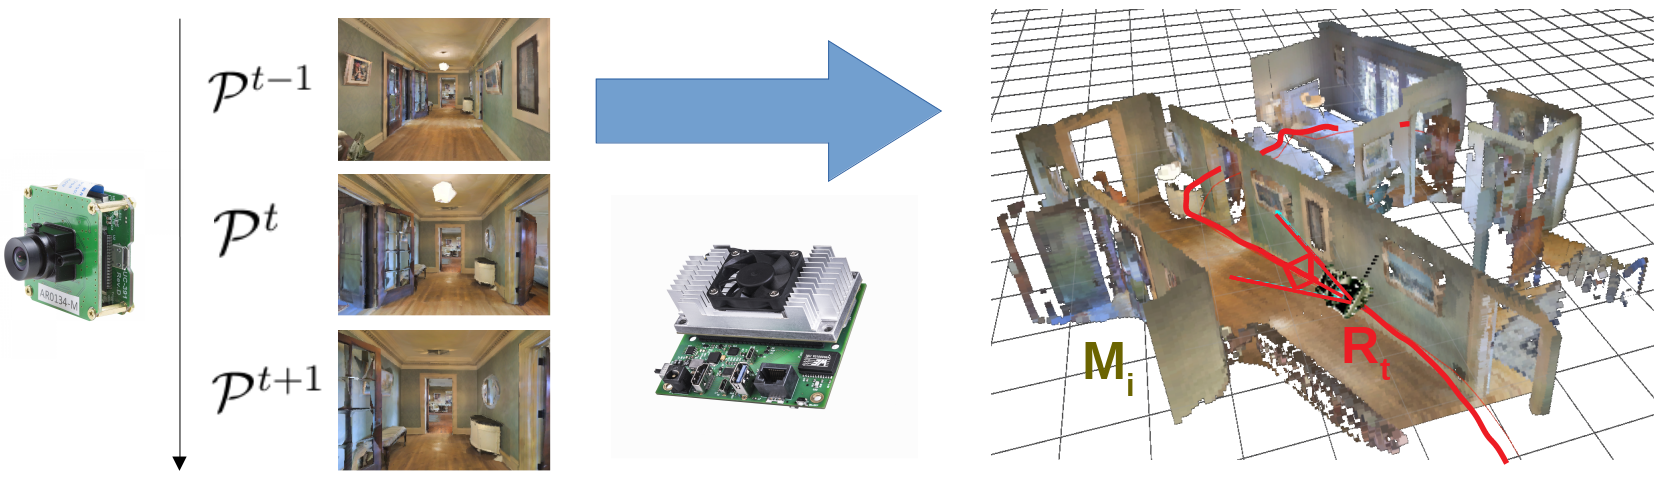
\includegraphics[width=1.0\textwidth]{img/vslam_problem_setting_1.png}
		\caption{Постановка задачи vSLAM}
		\label{figure_vslam_setting}
	\end{figure}
	
	Математически задачу можно сформулировать таким образом: существует набор точек в трёхмерном пространстве $\{M_i \} = \textbf{W}, M_i \in \mathbb{R}^3$, называемый сценой. Дана последовательность кадров $\{\mathcal{P}^t\}$. Каждый кадр является проекцией точек сцены с ракурса $\mathcal{R}_t = (x_t, y_t, z_t, p_t, r_t, w_t) \in \mathbb{R}^6$. Числа $x_t, y_t, z_t$ задают пространственное положение камеры в момент времени $t$, а $p_t, r_t, w_t$ - углы направления главной оптической оси камеры в момент времени $t$.
	
	Кадр представляется в виде трех матриц размер $H \times W$, содержащих числа от 0 до 1 - яркости соответствующих пикселей красной, синей и зеленой цветовых компонент:
	$$\mathcal{P}^t = \{\mathcal{P}^t_{c,h,w}\}_{c \in [1 \dots 3], h \in [1 \dots H], w \in [1 \dots W]} \in [0, 1]^{3 \times H \times W}$$
	Каждый элемент $c$-й матрицы кадра $\mathcal{P}^t_{c,h,w}$ представляет собой яркость $c$-й цветовой компоненты точки, которая в момент времени $t$ спроецировалась на позицию $(h, w)$ в матрице камеры:
	$$P(\mathcal{R}_t, M_i) = (h, w) \Rightarrow \mathcal{P}^t_{c,h,w} = I_c(\mathcal{R}_t, M_i),$$
	где $P(\mathcal{R}_t, M_i): \mathbb{R}^6 \times \mathbb{R}^3 \rightarrow \mathbb{R}^2$ - функция проекции точки пространства на матрицу камеры, принимающая на вход ракурс и положение точки в пространстве и возвращающая координаты проекции, а $I_c (\mathcal{R}_t, M_i): \mathbb{R}^6 \times \mathbb{R}^3 \rightarrow [0, 1]$ - функция яркости $c$-й цветовой компоненты точки $M_i$, рассматриваемой с ракурса $\mathcal{R}_t$.
	
	По имеющейся последовательности кадров $\{\mathcal{P}_t\}$ необходимо найти $(x_t, y_t, z_t)$ для всех моментов времени $t$ - координаты ракурсов $\mathcal{R}_t$, а также как можно большее количество координат точек $M_i$.
	
	\subsection{Одновременное картирование и локализация по видеоданным с картами глубины (RGBD-SLAM)}
	
	Задача одновременного картирования и локализации по видеоданным и данным глубины (RGBD-SLAM) возникает при навигации в неизвестной среде робота, имеющего на борту видеокамеру и сенсор глубины. Задача формулируется следующим образом: по изображениям с видеокамеры и картам глубины этих изображений необходимо построить трёхмерную модель окружающего пространства, и определить траекторию перемещения камеры в этом пространстве.
	
	Математически задачу можно сформулировать таким образом: существует набор точек в трёхмерном пространстве $\{M_i \} = \textbf{W}, M_i \in \mathbb{R}^3$, называемый сценой. Дана последовательность кадров $\{\mathcal{P}^t\}$ и карт глубины $\{\mathcal{D}^t\}$.
	
	Кадр представляется в виде трех матриц размер $H \times W$, содержащих числа от 0 до 1 - яркости соответствующих пикселей красной, синей и зеленой цветовых компонент:
	$$\mathcal{P}^t = \{\mathcal{P}^t_{c,h,w}\}_{c \in [1 \dots 3], h \in [1 \dots H], w \in [1 \dots W]} \in [0, 1]^{3 \times H \times W}$$
	Каждый элемент $c$-й матрицы кадра $\mathcal{P}^t_{c,h,w}$ представляет собой яркость $c$-й цветовой компоненты точки, которая в момент времени $t$ спроецировалась на позицию $(h, w)$ в матрице камеры:
	$$P(\mathcal{R}_t, M_i) = (h, w) \Rightarrow \mathcal{P}^t_{c,h,w} = I_c(\mathcal{R}_t, M_i)$$
	Карта глубины представляется в виде матрицы размера $H \times W$, содержащей положительные действительные числа - глубины соответствующих пикселей:
	$$\mathcal{D}^t = \{\mathcal{D}^t_{h,w}\}_{h \in [0 \dots H], w \in [0 \dots W]}$$
	Элемент матрицы карты глубины $D^t_{h,w}$ представляет собой расстояние от положения камеры в момент времени $t$ до точки, которая в момент времени $t$ спроецировалась на позицию $(h, w)$ в матрице камеры: 
	$$P(\mathcal{R}_t, M_i) = (h, w) \Rightarrow \mathcal{D}^t_{h,w} = \rho(M_i, (x_t, y_t, z_t))$$
	Здесь $P(\mathcal{R}_t, M_i): \mathbb{R}^6 \times \mathbb{R}^3 \rightarrow \mathbb{R}^2$ - функция проекции точки пространства на матрицу камеры, принимающая на вход ракурс и положение точки в пространстве и возвращающая координаты проекции, а $I_c (\mathcal{R}_t, M_i): \mathbb{R}^6 \times \mathbb{R}^3 \rightarrow [0, 1]$ - функция яркости $c$-й цветовой компоненты точки $M_i$, рассматриваемой с ракурса $\mathcal{R}_t$. Функция $\rho: \mathbb{R}^3 \times \mathbb{R}^3 \rightarrow \mathbb{R}_{+}$ задает евклидово расстояние между двумя точками в пространстве.
	
	\begin{figure}
		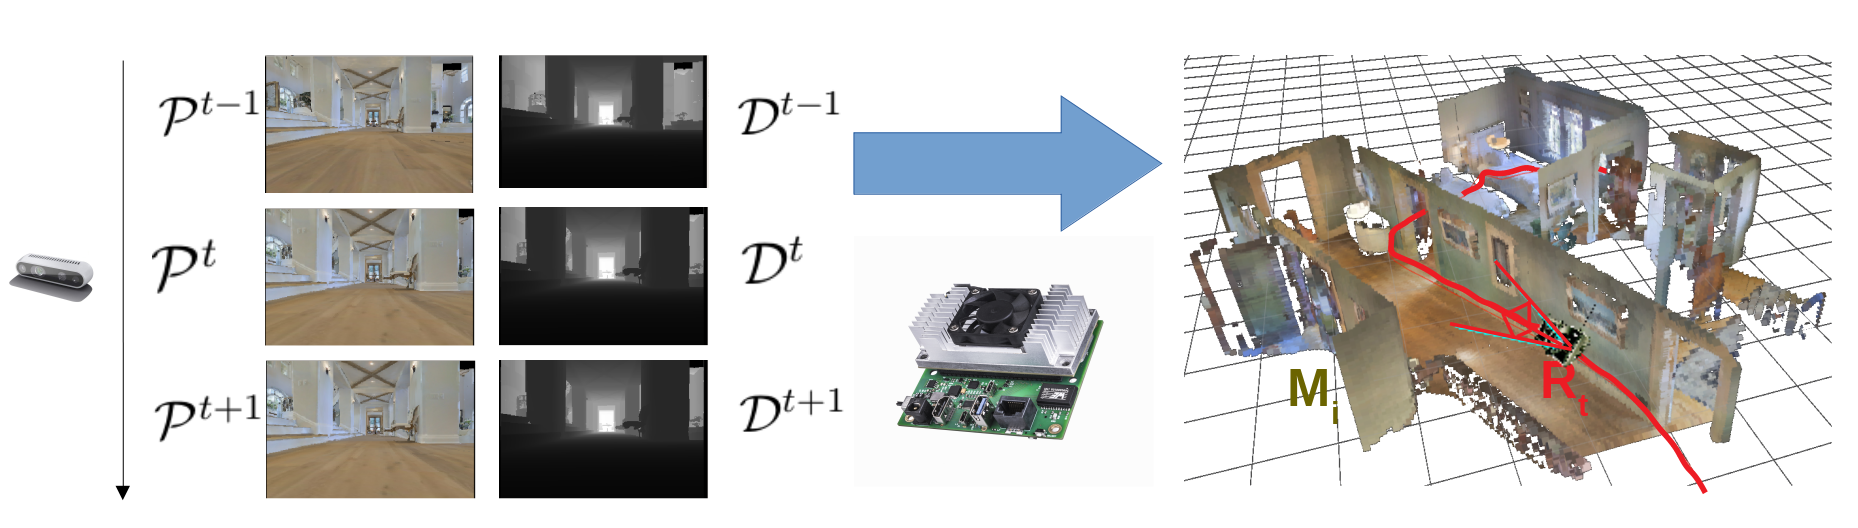
\includegraphics[width=1.0\textwidth]{img/rgbdslam_problem_setting_1.png}
		\caption{Постановка задачи RGB-D SLAM}
		\label{figure_rgbdslam_setting}
	\end{figure}
	
	По имеющейся последовательности кадров $\{\mathcal{P}_t\}$ и карт глубин $\{\mathcal{D}_t\}$ необходимо найти $(x_t, y_t, z_t)$ для всех моментов времени $t$ - координаты ракурсов $\mathcal{R}_t$, а также как можно большее количество координат точек $M_i$. Визуализация задачи RGB-D SLAM представлена на рисунке \ref{figure_rgbdslam_setting}.
	
	\subsection{Сведение RGBD-SLAM к vSLAM: восстановление карт глубин по видеопотоку}
	
	Задача восстановления карт глубин по видеопотоку возникает при навигации в неизвестной среде робота, не имеющего на борту никаких сенсоров, кроме видеокамеры. С помощью восстановления глубины по видеопотоку можно свести задачу vSLAM к задаче RGBD-SLAM, для которой разработаны более эффективные методы решения.
	
	\begin{figure}
		\centering
		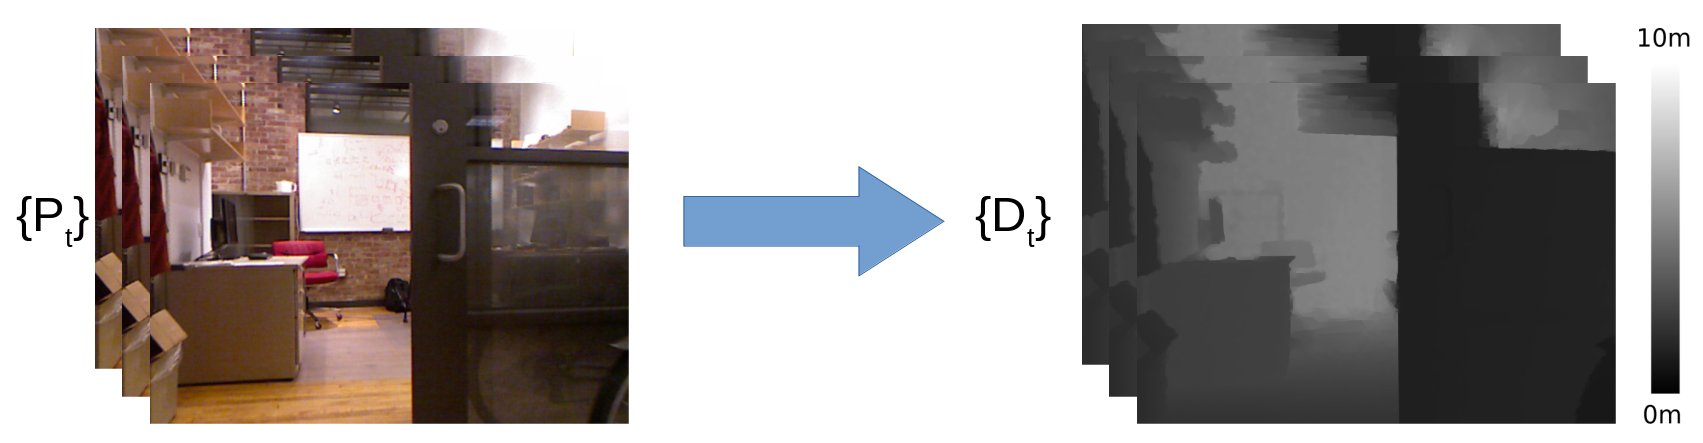
\includegraphics[width=1.0\textwidth]{img/de_problem_setting_1.png}
		\caption{Постановка задачи восстановления глубины}
		\label{figure_de_setting}
	\end{figure}
	
	Задача восстановления карт глубин по видеопотоку формулируется следующим образом: по изображениям, поступающим с единственной видеокамеры, необходимо определить расстояния до всех объектов, изображенных на этих изображениях (см. рис. \ref{figure_de_setting}). Математически задачу можно сформулировать таким образом: существует набор точек в трёхмерном пространстве $\{M_i \} = \textbf{W}, M_i \in \mathbb{R}^3$, называемый сценой. Дана последовательность кадров $\{\mathcal{P}^t\}$. Каждый кадр является проекцией точек сцены с ракурса $\mathcal{R}_t = (x_t, y_t, z_t, p_t, r_t, w_t) \in \mathbb{R}^6$. Числа $x_t, y_t, z_t$ задают пространственное положение камеры в момент времени $t$, а $p_t, r_t, w_t$ - углы направления главной оптической оси камеры в момент времени $t$.
	
	Кадр представляется в виде трех матриц размер $H \times W$, содержащих числа от 0 до 1 - яркости соответствующих пикселей красной, синей и зеленой цветовых компонент:
	$$\mathcal{P}^t = \{\mathcal{P}^t_{c,h,w}\}_{c \in [1 \dots 3], h \in [1 \dots H], w \in [1 \dots W]} \in [0, 1]^{3 \times H \times W}$$
	Каждый элемент $c$-й матрицы кадра $\mathcal{P}^t_{c,h,w}$ представляет собой яркость $c$-й цветовой компоненты точки, которая в момент времени $t$ спроецировалась на позицию $(h, w)$ в матрице камеры:
	$$P(\mathcal{R}_t, M_i) = (h, w) \Rightarrow \mathcal{P}^t_{c,h,w} = I_c(\mathcal{R}_t, M_i),$$
	где $P(\mathcal{R}_t, M_i): \mathbb{R}^6 \times \mathbb{R}^3 \rightarrow \mathbb{R}^2$ - функция проекции точки пространства на матрицу камеры, принимающая на вход ракурс и положение точки в пространстве и возвращающая координаты проекции, а $I_c (\mathcal{R}_t, M_i): \mathbb{R}^6 \times \mathbb{R}^3 \rightarrow [0, 1]$ - функция яркости $c$-й цветовой компоненты точки $M_i$, рассматриваемой с ракурса $\mathcal{R}_t$.
	
	По имеющейся последовательности кадров $\{\mathcal{P}_t\}$ необходимо для всех $h,w,t$ найти $\mathcal{D}^t_{h,w}$ - расстояния от положения камеры в момент $t$ до точек сцены, изображенных на кадре:
	$$P(\mathcal{R}_t, M_i) = (h, w) \Rightarrow \mathcal{D}^t_{h,w} = \rho((x_t, y_t, z_t), M_i)$$
	
	%----------------------------------------------------------------------------------------------------------------------
	% EVALUATION
	%-----------------------------------------------------------------------------------------------------------------------
	
	\section{Метрики качества}
	
	Для оценки качества алгоритмов одновременного картирования и локализации (vSLAM) и их сравнения между собой необходимо выбрать метрику оценки качества. Алгоритмы vSLAM, как правило, дают в качестве выходных данных карту окружающей местности и траекторию перемещения камеры. Качество построения карты и качество восстановления траектории, как правило, оценивается отдельно. Таким образом, метрики качества vSLAM подразделяются на две группы: метрики качества локализации и метрики качества картирования.
	
	\subsection{Метрики качества локализации}
	
	Метрики качества локализации, как правило, сравнивают траекторию, вычисленную алгоритмом SLAM, с истинной траекторией. Траектория представляет собой набор поз, каждая из которых включает трехмерную позицию (положение камеры в пространстве) и трехмерную ориентацию (направление главной оптической оси камеры). Оценка качества локализации сводится к вычислению ошибки между набором истинных и предсказанных поз. В научной литературе используются абсолютные и относительные ошибки, а также ошибки смещения и поворота.
	
	\begin{figure}
		\centering
		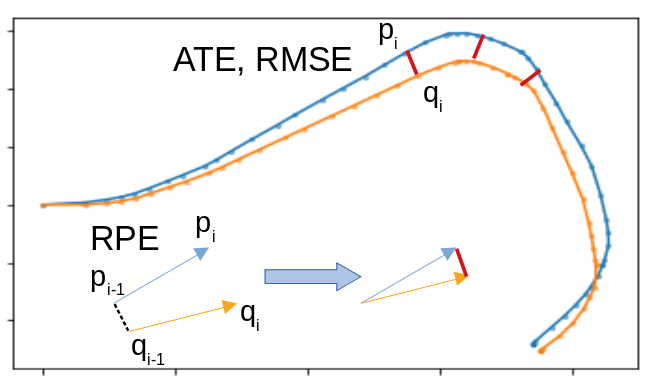
\includegraphics[width=0.7\textwidth]{img/localization_metrics.png}
		\caption{Схема вычисления абсолютной и относительной ошибки траектории}
		\label{figure_ate_rpe}
	\end{figure}
	
	Обозначим истинную траекторию как $\{(p_t, q_t)\}, t \in \{1, \dots, T\}$, где $p_t \in \mathbb{R}^3$ - трехмерная позиция камеры в момент времени $t$, $q_t \in \mathbb{R}^3$ - вектор направления главной оптической оси камеры в момент времени $t$. Предсказанную траекторию обозначим как $\{(\widehat{p_t}, \widehat{q_t})\}, t \in \{1, \dots, T\}$. Применяя различные функции ошибки к спискам поз $\{(p_t, q_t)\}$ и $\{(\widehat{p_t}, \widehat{q_t})\}$, можно вычислить абсолютную и относительную ошибку траектории (см. рис. \ref{figure_ate_rpe}).
	
	Абсолютная ошибка траектории (Absolute Trajectory Error, ATE) формулируется как среднеквадратичное отклонение точек предсказанной траектории от истинной:
	
	\begin{equation}
	\label{eq_ate}
	ATE = \sqrt{\frac{1}{T} \sum_{t=1}^T || p_t - \widehat{p_t} ||_2^2}
	\end{equation}
	
	Помимо абсолютной ошибки траектории, также широко применяется относительная ошибка позы (Relative Pose Error, RPE). Она формулируется как среднеквадратичное отклонение предсказанного смещения на каждом шаге от истинного:
	
	$$\Delta p_t = M_{q_{t-1}}^{-1} (p_t - p_{t-1});\ \Delta \widehat{p_t} = M_{\widehat{q_{t-1}}}^{-1} (\widehat{p_t} - \widehat{p_{t-1}})$$
	
	\begin{equation}
	\label{eq_rpe}
	RPE = \sqrt{\frac{1}{T} \sum_{t=1}^T ||\Delta p_t - \Delta \widehat{p_t} ||_2^2},
	\end{equation}
	
	где $M_{q_{t-1}}, M_{\widehat{q_{t-1}}}$ - матрицы вращения, переводящие вектор (1, 0, 0) в векторы $q_{t-1}$ и $\widehat{q_{t-1}}$ соответственно.
	
	В работе \cite{geiger2012we} приводятся следующие метрики качества локализации: относительное смещение и относительная ошибка поворота. Данные метрики учитывают не только расхождение между траекториями, но и их длину:
	
	\begin{equation}
	\label{eq_etrans}
	E_{trans} = \frac{1}{T} \sum\limits_{t=1}^T \frac{|| M_{q_{t-1}} (p_t - p_{t-1}) - M_{\widehat{q_{t-1}}} (\widehat{p_t} - \widehat{p_{t-1}}) ||_2}{|| p_t - p_{t-1} ||_2}
	\end{equation}
	
	\begin{equation}
	\label{eq_erot}
	E_{rot} = \frac{1}{T} \frac{\angle(M_{q_{t-1}} (p_t - p_{t-1}), M_{\widehat{q_{t-1}}} (\widehat{p_t} - \widehat{p_{t-1}}))}{|| p_t - p_{t-1} ||_2}
	\end{equation}
	
	\subsection{Метрики качества картирования}
	\label{section_our_ame}
	
	Оценка качества картирования является более сложной задачей, чем оценка качества локализации. Если при оценке качества локализации легко установить соответствия между точками истинной и предсказанной траекторий (по времени прохождения данных точек), то явного соответствия между точками истинной и предсказанной карты не существует. Как правило, соответствия устанавливаются методом ближайшего соседа - каждая точка предсказанной карты сопоставляется с ближайшей к ней точкой истинной карты. Такой подход применяется в программном пакете CloudCompare\footnote{http://cloudcompare.org/} и в работах \cite{handa2014benchmark}\cite{wasenmuller2016corbs}. Применяя среднеквадратичную ошибку (RMSE) в этом подходе, получаем абсолютную ошибку картирования (Absolute Mapping Error, AME).
	
	По заданной истинной карте, представленной в виде трехмерного облака точек:
	
	\begin{equation}
	M=\{m_i \in \mathbb{R}^3; i \in [1;n]; n \in \mathbb{N}\}
	\label{eq_gt_map}
	\end{equation}
	
	и карте, построенной алгоритмом vSLAM:
	
	\begin{equation}
	M^*=\{m^*_j \in \mathbb{R}^3; j \in [1;N]; n \in \mathbb{N}\}
	\label{eq_vslam_map}
	\end{equation}
	
	абсолютная ошибка картирования вычисляется следующим образом:
	
	$$j' = \arg\min\limits_{i} ||m^*_j - m_{i}||_2$$
	
	\begin{equation}
		\label{eq_ame}		
		AME(M, M^*) = \sqrt{\frac{1}{N} \sum\limits_{j=1}^N ||m^*_j  - m_{j'}||_2^2}
	\end{equation}
	
	\begin{figure}
		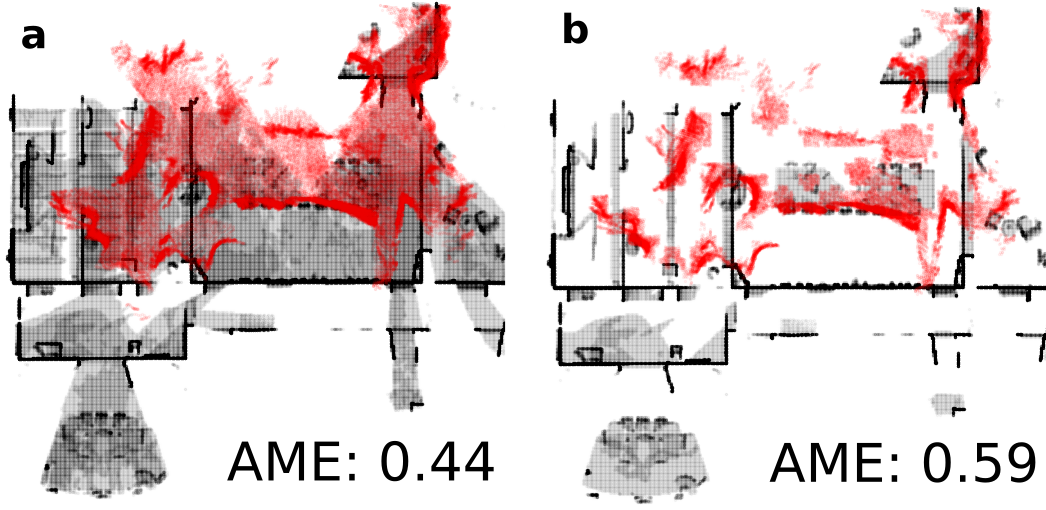
\includegraphics[width=1.0\textwidth]{img/1_first_paired.png}
		\caption{Исходные карты (a) и карты с вырезанным полом (b). Черным отмечены точки истинной карты, красным - предсказанной методом vSLAM карты. Метрика AME на картах с полом значительно ниже, чем на тех же картах без пола.}
		\label{figure_floor}
	\end{figure}
	
	Однако существуют ситуации, когда абсолютная ошибка картирования, вычисленная по методу ближайшего соседа, не является репрезентативной. Например, при картировании помещений большой площади точки стен предсказанной карты могут быть сопоставлены с точками пола истинной карты. Таким образом абсолютная ошибка картирования может быть небольшой даже при неточном картировании. Так получилось в одном из экспериментов, описанных в разделе \ref{section_experiments}. При картировании помещений алгоритмом SLAM с глубинами, предсказанными нейросетью, обнаружилось, что карты визуально получались довольно неточные, при этом значение метрики AME на этих картах оказалось низким. При удалении точек пола из истинных и предсказанных карт значение метрики AME существенно выросло (см. рис. \ref{figure_floor}). Таким образом, в контексте оценки качества алгоритмов vSLAM метрика AME с сопоставлением по методу ближайшего соседа малоприменима.
	
	В данной работе для оценки качества картирования предлагается использовать способ сопоставления точек истинной и предсказанной карты, описанный в работе \cite{bokovoy2021assessment}. Предлагаемый способ основан на сопоставлении ракурсов, с которых видны точки истинной и предсказанной карт. Ниже приведено его подробное описание.
	
	\begin{figure}
		%\centering
		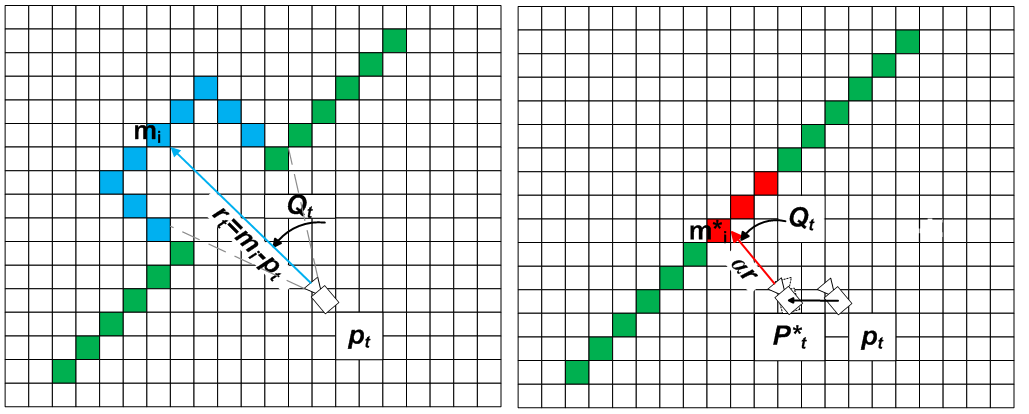
\includegraphics[width=1.0\textwidth]{img/corresp.png}
		\caption{Пример сопоставления точек истинной и предсказанной карты с использованием ракурса. Источник \cite{bokovoy2021assessment}}
		\label{figure_correspondences}
	\end{figure}
	
	Пусть $M,\ M^*$ - истинная и построенная алгоритмом vSLAM карты (\ref{eq_gt_map}, \ref{eq_vslam_map}); $m_i^*$ - точка карты $M^*$, попадающая в поле зрения камеры в момент времени $t$; $p_t^*, q_t^*$ - предсказанные методом vSLAM положение и ориентация камеры в момент времени $t$; $p_t, q_t$ - истинные положение и ориентация камеры в момент $t$. Нужно построить функцию $f: M^* \longrightarrow M$, устанавливающую соответствие между точками построенной и истинной карты.
	
	Обозначим матрицы вращения, заданные ориентациями $q_t$ и $q_t^*$, как $M_{q_t}$ и $M_{q_t^*}$ соответственно. Вектор $r_t = (M_{q_t^*})^{-1} M_{q_t} (m_i^* - p_t)$ соответствует направлению с позиции камеры на точку $m_i^*$ в истинной карте (точка $p_t + \alpha r_t$ в истинной карте будет видна в момент $t$ под тем же ракурсом, что точка $m_i^*$ в предсказанной карте, см. рис. \ref{figure_correspondences}). Точке $m_i^*$ будет сопоставлена ближайшая точка истинной карты, которая видна под таким ракурсом:
	
	\begin{equation}
	\label{eq_corresp_function}
	f(m_i^*) = p_t + \alpha r_t;\ \ \alpha = \arg\min \limits_{\alpha'}: p_t + \alpha' r_t \in M
	\end{equation}

	Абсолютная и относительная ошибки картирования с таким методом сопоставления будет выглядеть следующим образом:
	
	\begin{equation}
		\label{eq_ame_our}
		AME(M, M^*) = \sqrt{\frac{1}{N} \sum\limits_{i=1}^N ||m_i^* - f(m_i^*)||_2^2}
	\end{equation}
	
	\begin{equation}
	\label{eq_rme_our}
	RME(M, M^*) = \sqrt{
	\begin{aligned}
	\frac{1}{N} \sum\limits_{i=1}^N ||M_{q_t^*}^{-1}(m_i^* - p_t^*) - \\
		- M_{q_t}^{-1} (f(m_i^*) - p_t)||_2^2
	\end{aligned}
	}
	\end{equation}
	
	При использовании данных метрик возникает следующая проблема. Одна точка карты может быть видна с разных позиций (т.е. для одной точки $m_i^*$ есть несколько $t$, по которым можно построить разные соответствия). Поэтому нужно определиться со способом выбора $t$. Наиболее целесообразными выглядят следующие варианты:
	
	\begin{itemize}
		\item $t$ выбирается как момент, в который точка $m_i^*$ попала в поле зрения камеры в первый раз;
		\item $t$ выбирается как момент, в который точка $m_i^*$ попала в поле зрения камеры в последний раз;
		\item $t$ выбирается как момент видимости точки $m_i^*$, в который точка была наиболее близка к позиции камеры;
		\item $t$ рассматриваются все моменты $t$, в который точка попадала в поле зрения камеры; при вычислении метрики берется усредненное расстояние между точкой $m_i^*$ и точками $f(m_i^*, t)$ для всех $t$.
	\end{itemize}

	Последний вариант выбора $t$ приводит к большим вычислительным затратам, однако метрика с ним получается наиболее стабильной. Для оценки качества алгоритмов vSLAM в данной работе был выбран именно этот вариант.
	
	Метрики AME и RME, вычисленные на основе функции сопоставления $f$, являются более подходящими для оценки качества алгоритмов vSLAM, поскольку они учитывают не только расстояния между точками, но и процесс построения карты алгоритмом vSLAM. Также данные метрики являются более устойчивыми к различным изменениям структуры карты (например, удаление точек пола), что подтверждено экспериментами, описанными в разделе \ref{section_experiments}.
	
	\section{Коллекции данных}
	
	 Проведение натурных экспериментов на реальной робототехнической системе затратно, а повторяемость таких экспериментов затруднена, поэтому для тестирования алгоритмов vSLAM и их сравнения между собой обычно применяются предварительно собранные коллекции данных. Такие коллекции должны включать в себя запись видеопотока с камеры робота (в случае RGB-D камеры - запись изображений и данных о глубине), а также данные об истинных позициях робота и истинной карте окружающей местности для вычисления метрик качества. Подобные коллекции бывают двух видов: собранные в реальном мире и синтетические.
	 
	 При сборке коллекций данных в реальном мире возникают сложности с определением истинной траектории робота и точной модели окружающей местности. Для вычисления точных данных о движении робота и его окружающей среде необходимо редкое и дорогостоящее оборудование, а также значительные временные затраты. Как правило, в коллекциях данных из реального мира имеются данные лишь о траектории робота, собранные с помощью систем отслеживания движения (Motion-capture System \cite{kurihara2002optical}), а истинные карты окружающей среды отсутствуют. При тестировании методов vSLAM на таких коллекциях можно вычислить метрики ATE \ref{eq_ate}, RPE \ref{eq_rpe}, $E_{trans}$ \ref{eq_etrans}, $E_{rot}$ \ref{eq_erot}, но невозможно вычислить метрики AME и RME (\ref{eq_ame}, \ref{eq_ame_our}, \ref{eq_rme_our}).
	 
	 Синтетические коллекции данных, а также различные робототехнические симуляторы (например, \cite{koenig2004design} \cite{rooban2021coppeliasim}) позволяют легко получить истинные карты и траектории, однако в большинстве обладают низкой фотореалистичностью, что критически важно для алгоритмов визуального картирования и локализации.
	
	\subsection{Коллекции данных из реального мира}
	
	Коллекции данных, собранные с помощью прогонов системы, оснащенной камерой, по некоторой траектории в реальном мире, на данный момент очень широко распространены. Имеется множество коллекций, в которых представлены прогоны робота в помещениях, а также несколько крупных коллекций, собранных с автомобиля, оснащенного большим количеством датчиков. В большинстве таких коллекций представлены истинные траектории движения робота, но отсутствуют истинные карты окружающей местности. Подобные датасеты хорошо подходят для оценки качества локализации методов vSLAM, однако оценка качества картирования на них затруднена или вовсе невозможна. Ниже представлен обзор наиболее широко используемых наборов данных из реального мира для тестирования vSLAM.
	
	Одним из самых известных датасетов для тестирования алгоритмов SLAM является KITTI \cite{geiger2012we}. Он содержит 22 сцены, записанные с автомобиля в городской среде. Общая длина проезда составляет 39 км. Датасет содержит порядка 41 тысячи кадров видеопотока, записанного со стереокамеры, а также данные трехмерного лазерного сканера (лидара) и инерциальной навигационной системы (ИНС) совместно с показаниями GPS. В данной коллекции также представлены истинные позиции, вычисленные с помощью агрегации данных GPS и ИНС и качественной пост-обработки. Истинная карта окружающих объектов не представлена, однако она может быть приблизительно воссоздана по истинным позициям автомобиля и облакам точек с лидара.
	
	Помимо исходных данных с сенсоров, в KITTI также представлено программное обеспечение, необходимое для вычисления метрик качества локализации. Также в датасете предоставлены данные для тестирования некоторых других методов компьютерного зрения: семантической сегментации, детекции объектов, вычисления оптического потока. Данный датасет широко используется для оценки качества методов визуальной одометрии \cite{geiger2015kitti}, а также для обучения различных нейросетевых моделей \cite{li2018megadepth} \cite{zhou2017unsupervised} \cite{patil2020don}. Однако оценка качества картирования на данном датасете затруднительна, поскольку истинных карт окружающей среды в датасете не предоставлено.
	
	Одним из наиболее широко используемых датасетов для тестирования vSLAM в помещениях является RGB-D SLAM dataset and benchmark \cite{sturm2012benchmark}, созданный учеными из Технического университета Мюнхена (TUM). Датасет содержит 39 последовательностей, записанных в различных помещениях с камеры Microsoft Kinect \cite{zhang2012microsoft}, установленной на малом колесном роботе. Последовательности были записаны в различных помещениях, длины траекторий не превосходят 40 метров. Помимо изображений и карт глубины с камеры Kinect, в датасете также имеются истинные траектории проезда робота, вычисленные с помощью высокоточной системы отслеживания движения (Motion Capture System).
	
	Датасет от TUM также содержит набор программного обеспечения для тестирования алгоритмов SLAM и вычисления метрик ATE (\ref{eq_ate}) и RPE (\ref{eq_rpe}). Благодаря набору ПО, а также наличию истинных траекторий, данный датасет хорошо подходит для оценки качества локализации методов vSLAM и RGB-D SLAM в помещениях. Однако оценка качества картирования на нем невозможна, так как не представлены истинные координаты точек окружающих объектов. Обучение нейронных сетей на данной коллекции затруднительно из-за ее небольшого объема, а также однообразности изображений.
	
	Еще одним широко используемым для тестирования vSLAM датасетом является EuRoC \cite{burri2016euroc}. В этом датасете представлены данные с видеокамеры, установленной на квадрокоптере, собранные с 11 прогонов по двум комнатам. Помимо видеоданных, также имеются данные ИНС и истинные траектории квадрокоптера, измеренные с помощью системы отслеживания движения (Motion Capture System). Карт глубины датасет не содержит, поэтому он не подходит для оценки качества алгоритмов RGB-D SLAM. Программного обеспечения для запуска алгоритмов vSLAM и вычисления метрик разработчики также не предоставили. Ввиду всего вышеперечисленного применимость данного датасета для оценки качества методов vSLAM весьма ограниченна.
	
	В настоящее время существуют также коллекции данных, в которых помимо траекторий предоставлены трехмерные модели окружающих объектов, что дает возможность оценить не только качество локализации, но и качество картирования. Одной из самых крупных таких коллекций является ScanNet \cite{dai2017scannet}. В данной коллекции представлены 2.5 млн пар изображение-глубина, снятые RGB-D камерами в 1513 помещениях. Траектории камеры и трехмерные модели помещений были получены с помощью тщательной алгоритмической обработки данных RGB-D камеры и ИНС. Сенсоры, использованные при создании датасета, имеют достаточно большую погрешность, поэтому полученные таким образом траектории и карты сложно считать ``истинными''. При проведении экспериментов с методами vSLAM возможны искажения оценок их качества.
	
	Датасет ScanNet изначально не предназначался для тестирования алгоритмов vSLAM, и в нем не предоставлено нужного для этого программного обеспечения и удобного формата данных. Поэтому тестирование методов vSLAM на данном датасете весьма затруднительно. Однако датасет может быть полезен для решения вспомогательных задач для visual SLAM - например, обучения нейросетей восстановления глубины и визуальной одометрии.
	
	\subsection{Симуляторы и коллекции синтетических данных}
	\label{section_synthetic_datasets}
	
	Благодаря бурному развитию вычислительной техники и компьютерных технологий, в последние годы были разработаны различные робототехнические симуляторы. Появление симуляторов дало широкие возможности для тестирования робототехнических алгоритмов, в том числе методов картирования и локализации. В симуляционной среде робот может перемещаться по произвольной траектории, для которой всегда известны истинные позиции, что дает возможность проведения неограниченного числа экспериментов по оценке качества методов SLAM.
	
	Наиболее применяемыми на данный момент симуляторами являются Gazebo \cite{koenig2004design} и CoppeliaSim (V-REP) \cite{rooban2021coppeliasim}. Эти симуляторы отличаются подробным моделированием различных физических процессов, благодаря чему в них можно имитировать работу различных сенсоров, таких, как ИНС и лазерные сканеры, а также видеокамер и RGB-D камер. Однако фотореалистичность интерьеров в подобных симуляторах довольно низкая (см. рис. \ref{figure_gazebo_vrep}) - из-за повторяемости текстур и неточного моделирования распространения света могут возникнуть проблемы с тестированием алгоритмов Visual SLAM.
	
	\begin{figure}
		\centering
		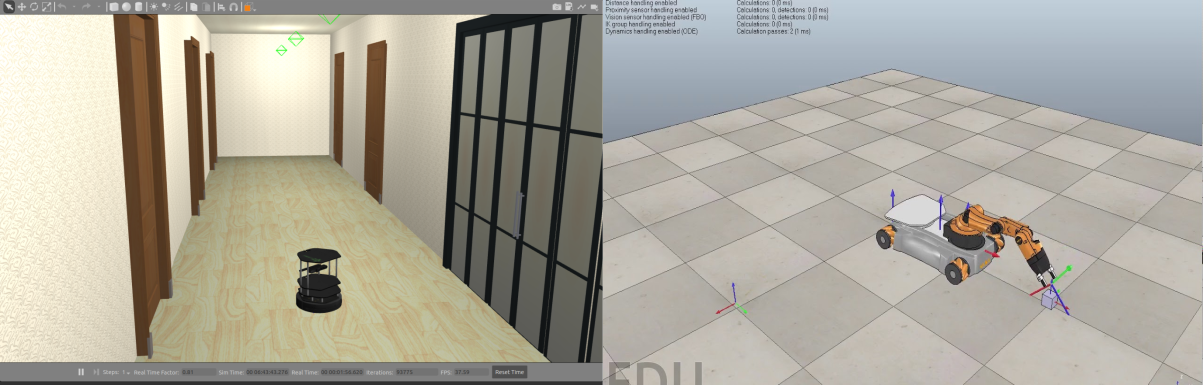
\includegraphics[width=0.9\textwidth]{img/gazebo_vrep.png}
		\caption{Пример симуляционной среды Gazebo (слева) и CoppeliaSim (справа). Однообразность текстур делает работу методов Visual SLAM затруднительной}
		\label{figure_gazebo_vrep}
	\end{figure}

	\begin{figure}
		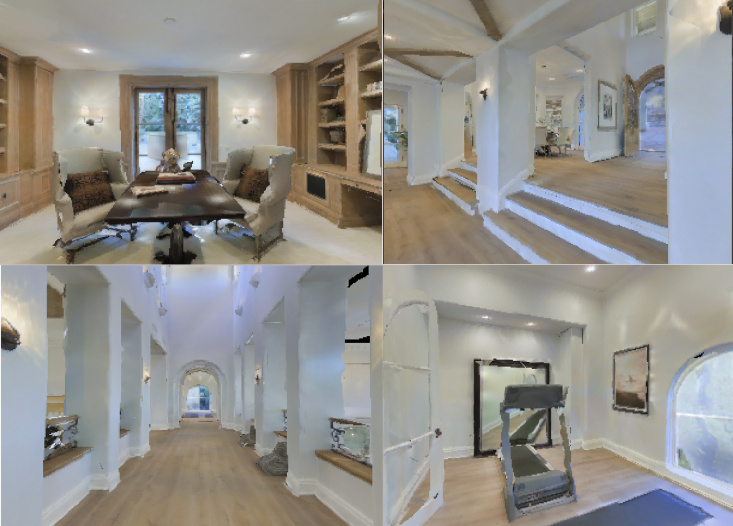
\includegraphics[width=0.9\textwidth]{img/habitat.png}
		\caption{Пример изображений с камеры робота в симуляционной среде Habitat на сцене из датасета Matterport3D}
		\label{figure_habitat}
	\end{figure}
	
	Проблемы фотореалистичности частично решились с появлением симулятора Habitat \cite{savva2019habitat}. В данном симуляторе не моделируются такие физические процессы, как инерция движения и распространение лазерных лучей, однако изображения сцен, используемые в нем, отличаются высокой фотореалистичностью (см. рис. \ref{figure_habitat}). Как правило, в симуляторе Habitat используются сцены из коллекции Gibson \cite{xia2018gibson} или Matterport3D \cite{chang2017matterport3d}. Их фотореалистичность обусловлена тем, что сцены построены по реальным помещениям с помощью специальной камеры\footnote{https://matterport.com/} и тщательной алгоритмической пост-обработки. Коллекция Matterport3D содержит около 60 сцен площадью в несколько сотен квадратных метров каждая. Коллекция Gibson содержит около 500 сцен площадью несколько десятков квадратных метров каждая. В обоих коллекциях представлены здания и помещения различного типа. Симуляционная среда дает возможность перемещаться в этих помещениях по произвольной траектории.
	
	В рамках данной работы на основе симулятора Habitat и коллекции сцен Matterport3D был собран новый датасет для оценки качества алгоритмов vSLAM. Датасет содержит 40 траекторий, которые разделены на 20 перекрывающихся пар, что дает возможность также тестировать алгоритмы объединения карт (Map Merging). Длины траекторий варьируются от 4 до 33 метров. В датасете представлены RGB-D данные (суммарно около 30000 пар картинка-глубина), а также истинные траектории перемещения камеры и истинные карты помещений, построенные с помощью метода обратной проекции по истинным позициям и точным картам глубин. Подробное описание собранного датасета доступно в работе \cite{bokovoy2021maomaps}. Эксперименты по оценке качества методов vSLAM на нем описаны в разделе \ref{section_experiments}.
	
	%------------------------------------------------------------------------------------------------------------------------
	% METHODS
	%------------------------------------------------------------------------------------------------------------------------
	
	\chapter{Методы решения задачи vSLAM}
	
	\section{Классические методы}
	
	Как правило, для решения задачи vSLAM применяются методы, основанные на вычислении геометрических преобразований между позициями камеры по изображениям. Преобразования могут вычисляться как прямыми методами (например, минимизацией фотометрической ошибки), так и путем сопоставления извлеченных из изображений особых точек. По вычисленным преобразованиям восстанавливается траектория перемещения камеры. Также с использованием этих преобразований обычно строятся локальные карты - карты участка местности, попадающего в поле зрения камеры, которые затем соединяются в глобальную карту с помощью различных вероятностных методов.
	
	В настоящее время существует множество алгоритмов vSLAM \cite{taketomi2017visual} \cite{fuentes2015visual}. В данной работе представлен обзор методов vSLAM, предназначенных для работы в реальном времени в условиях ограниченных вычислительных ресурсов и имеющих открытый исходный код.
	
	\subsection{ORB-SLAM и ORB-SLAM2}
	
	Алгоритм ORB-SLAM \cite{mur2015orb} и его модификация ORB-SLAM2 \cite{mur2017orb} являются одними из наиболее популярных методов одновременного картирования и локализации. ORB-SLAM использует в качестве входных данных видеопоток с единственной камеры, а ORB-SLAM2 является расширением алгоритма для работы по данным стереокамеры или RGB-D камеры. В основе алгоритма лежит извлечение особых точек из изображений с помощью детектора ORB \cite{rublee2011orb}. Высокая скорость детектора ORB позволяет методу работать в реальном времени в условиях ограниченных вычислительных ресурсов. Однако на карту наносятся лишь координаты особых точек, поэтому построенная алгоритмом карта получается разреженной (см. рис. \ref{figure_orb_slam_map}) и является непригодной для планировния траектории (планировщик может проложить маршрут между двумя особыми точками, где может быть стена или другое препятствие).

	\begin{figure}
		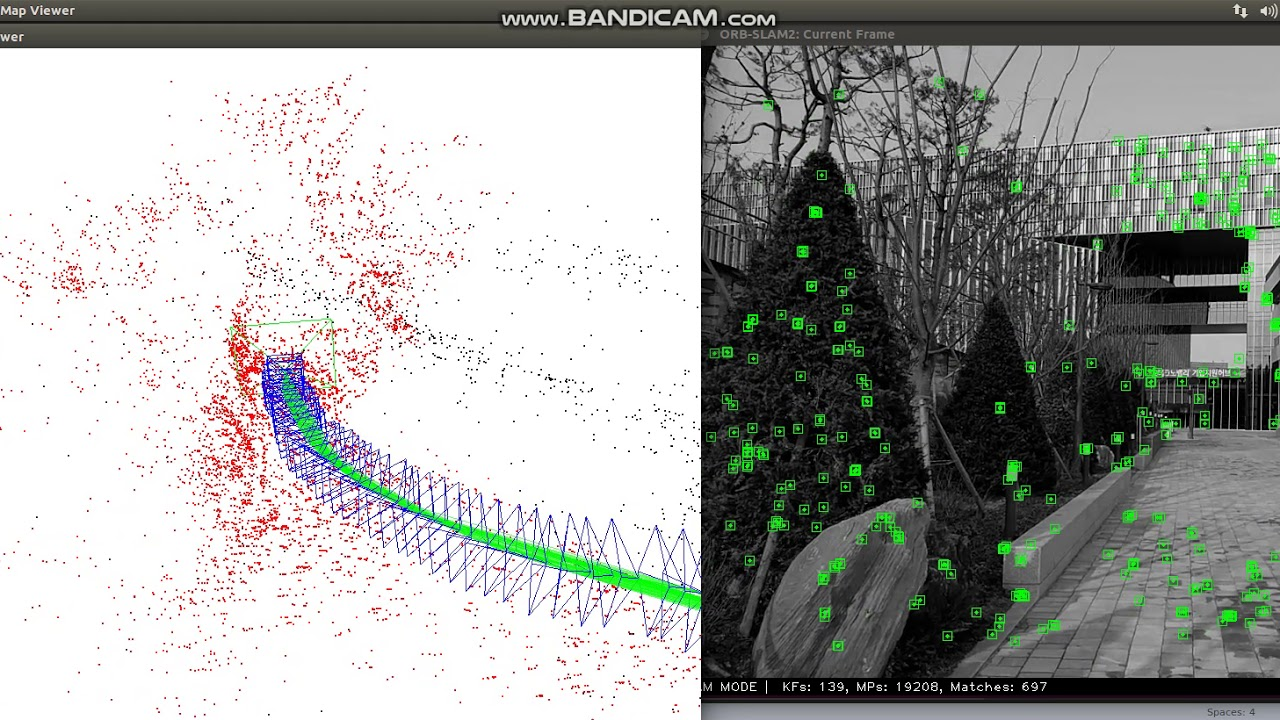
\includegraphics[width=1.0\textwidth]{img/orb_slam_map.jpg}
		\caption{Работа алгоритма ORB-SLAM: построенная карта (слева) и детекция особых точек на изображении (справа). Карта представляет собой сильно разреженный набор точек, что затрудняет навигацию в ней. Источник: \url{https://www.youtube.com/watch?v=g_nFyS0muJw}}
		\label{figure_orb_slam_map}
	\end{figure}

	\begin{figure}
		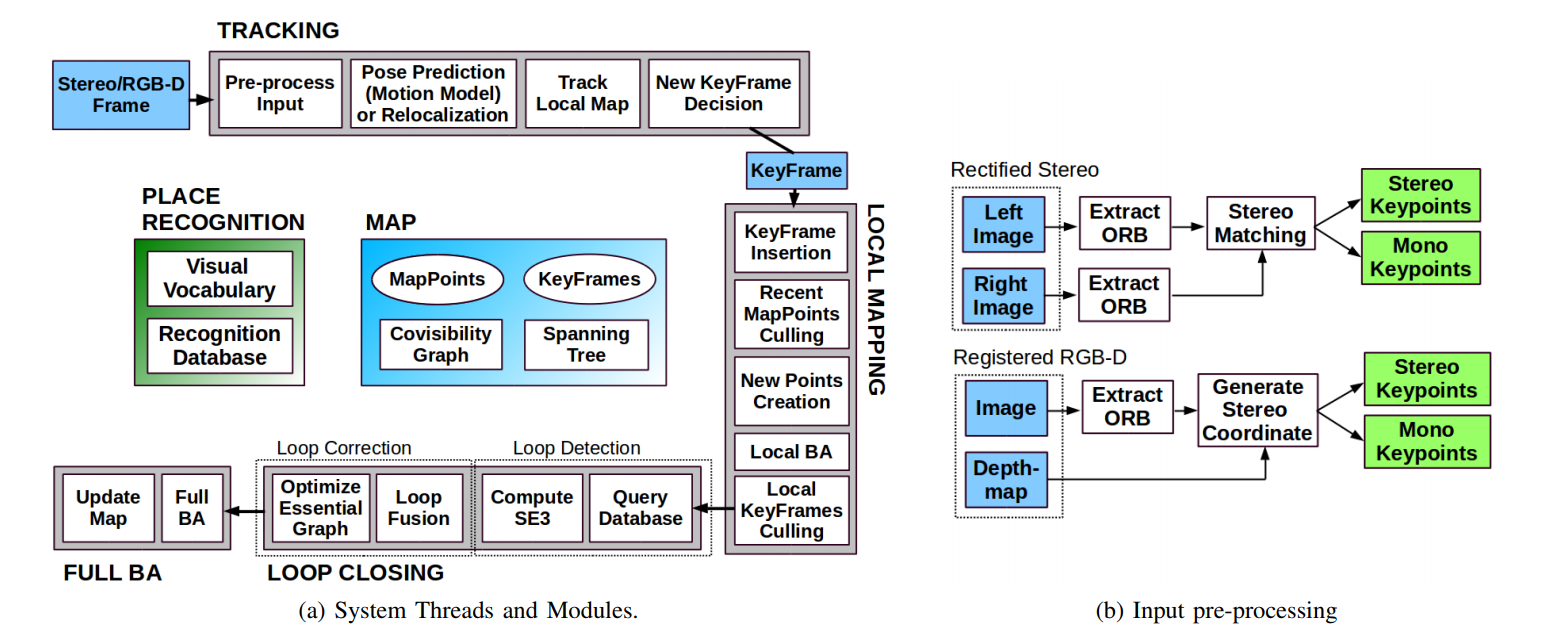
\includegraphics[width=1.0\textwidth]{img/orb_slam_scheme_high_resolution.png}
		\caption{Схема алгоритма ORB-SLAM. Источник \cite{mur2015orb}}
		\label{figure_orb_slam}
	\end{figure}
	
	Работа алгоритма ORB-SLAM разделена на три основных потока, выполняющихся параллельно:
	
	\begin{itemize}
		\item Tracking - отслеживание кадров. Данный поток приблизительно определяет текущее положение камеры с помощью поиска похожего кадра и сопоставления особых точек на нем и текущем кадре.
		\item Local Mapping - построение и оптимизация локальной карты (вблизи текущего положения камеры).
		\item Loop Closing - поиск и замыкание циклов с помощью объединения похожих кадров.
	\end{itemize}

	Схема основных компонентов алгоритма изображена на рисунке \ref{figure_orb_slam}.
	
	\subsection{LSD-SLAM}
	
	Алгоритм LSD-SLAM \cite{engel2014lsd} так же, как и ORB-SLAM, выполняет картирование и локализацию по данным с единственной камеры, однако он имеет другой принцип действия. Траектория перемещения камеры вычисляется не сопоставлением особых точек, а путем минимизации фотометрической ошибки по всему изображению. Благодаря использованию полного изображения вместо набора особых точек, LSD-SLAM строит более плотную карту, однако при этом он имеет более высокие требования к вычислительным ресурсам, чем ORB-SLAM. При работе алгоритма LSD-SLAM в реальном времени на маломощном вычислительном устройстве могут возникнуть проблемы. Недостатками данного алгоритма также являются высокие требования к калибровке камеры и неустойчивость к выбросам.
	
	\begin{figure}
		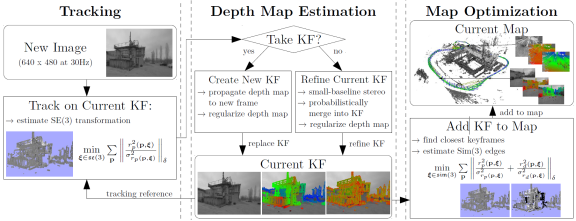
\includegraphics[width=1.0\textwidth]{img/lsd_slam_scheme.png}
		\caption{Схема алгоритма LSD-SLAM. Источник \cite{engel2014lsd}}
		\label{figure_lsd_slam}
	\end{figure}
	
	Алгоритм LSD-SLAM состоит из трех основных модулей: tracking, depth map estimation и map optimization. Схема алгоритма представлена на рисунке \ref{figure_lsd_slam}.
	
	Модуль \textbf{tracking} определяет перемещение камеры, отслеживая входящие изображения и вычисляя преобразование подобия между ними. Для вычисления преобразования используется минимизация фотометрической ошибки между новым изображением и преобразованным текущим ключевым кадром.
	
	Модуль \textbf{depth map estimation} сравнивает кадр с текущим ключевым кадром, а затем уточняет или полностью заменяет его. Для сравнения используется взвешенная сумма расстояний и углов поворота между кадрами. Если она больше некоторого порога, ключевой кадр заменяется новым. По ключевому кадру вычисляется инвертированная карта глубины путем сопоставления точек с предыдущим ключевым кадром с использованием преобразнвания подобия, вычисленного модулем tracking. По вычисленному местоположению камеры и инвертированным картам глубины строится карта окружающей местности.
	
	Модуль \textbf{map optimization} выполняет оптимизацию карты с использованием библиотеки g2o \cite{grisetti2011g2o}. Оптимизация позволяет предотвратить накопление ошибок вычисления траектории и поддерживает точность построения карты.
	
	Для хранения карты окружающей среды используется граф. Каждый узел этого графа хранит соответствующий ключевой кадр и инвертированную карту его глубины. Узлы соединяются ребрами, содержащими преобразование подобия между кадрами.
	
	\subsection{RTAB-MAP}
	\label{section_rtabmap}
	
	Алгоритм RTAB-MAP \cite{labbe2019rtab} предназначен для решения задачи SLAM с использованием информации о глубине изображений (по данным видеокамеры и лидара, или RGB-D камеры, или стереопары камер). Алгоритм использует три независимых процесса: вычисление движения камеры (одометрии), картирование и замыкание циклов. Схема алгоритма представлена на рисунке \ref{figurertabmap}.
	
	\begin{figure}
		\centering
		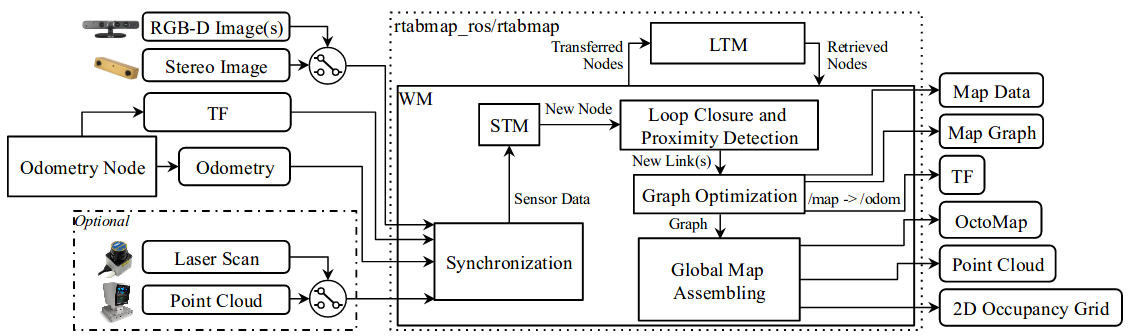
\includegraphics[scale=0.4]{img/rtabmap_scheme.png}
		\caption{Общая схема алгоритма RTAB-Map}
		\label{figurertabmap}
	\end{figure}
	
	Для одометрии по кадрам вычисляются особые точки с помощью детектора BRIEF \cite{calonder2010brief}. По сопоставлению особых точек на текущем и ключевом кадрах с помощью алгоритма PnP RANSAC \cite{brachmann2017dsac} вычисляется перемещение камеры. Полученное положение камеры корректируется с помощью алгоритма Local Bundle Adjustment \cite{zhang2006incremental} и предсказаний на основе предыдущих движений камеры. Новый ключевой кадр добавляется, когда у текущего кадра и ключевого будет мало сопоставлений. Схема вычисления одометрии представлена на рисунке \ref{figurergbdodometry}.
	
	\begin{figure}
		\centering
		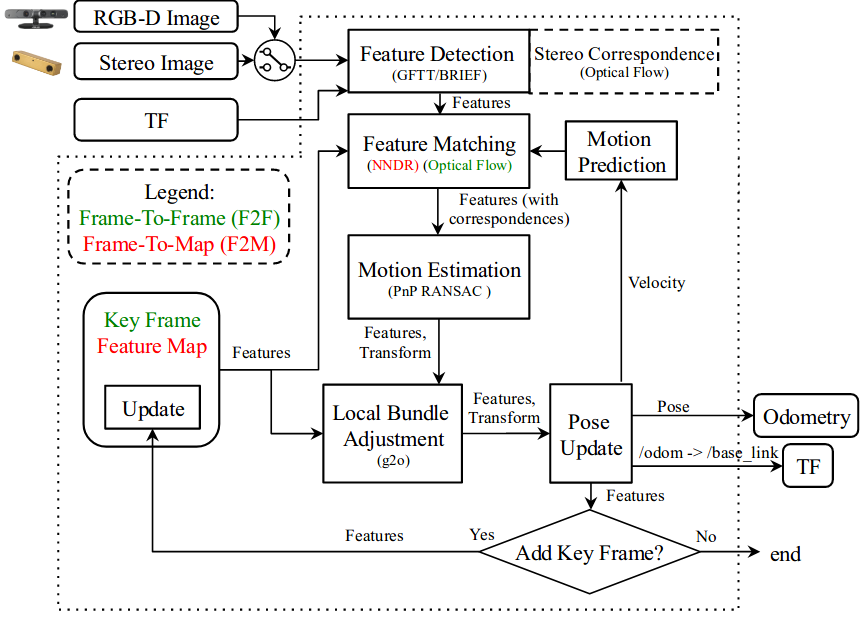
\includegraphics[scale=0.4]{img/rgbd_odometry.png}
		\caption{Схема вычисления одометрии в методе RTAB-Map. Источник \cite{labbe2019rtab}}
		\label{figurergbdodometry}
	\end{figure}
	
	Картирование выполняется по локальным сеткам заполненности (occupancy grid), полученных из карт глубины. Локальные карты с помощью воксельного фильтра сшиваются в глобальную карту. При замыкании цикла карта перестраивается. Схема процесса построения карты по локальным облакам точек представлена на рисунке \ref{figuremapping}.
	
	\begin{figure}
		\centering
		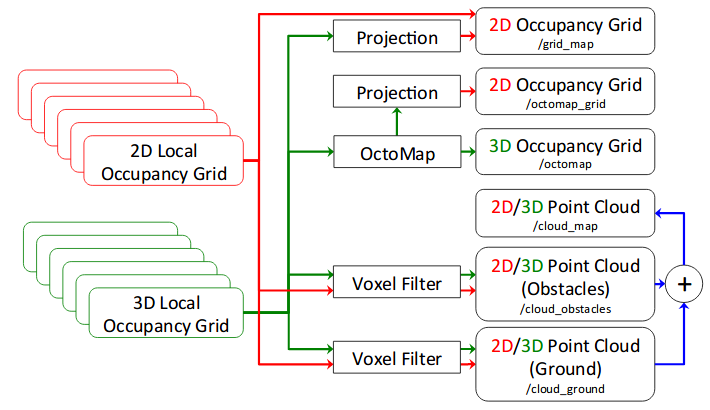
\includegraphics[scale=0.5]{img/rtabmap_mapping.png}
		\caption{Схема построения плотной глобальной карты по локальным сеткам. Источник \cite{labbe2019rtab}}
		\label{figuremapping}
	\end{figure}
	
	Замыкание циклов основывается на сопоставлении особых точек на кадрах с видеопотока. Ключевая особенность данного метода - эффективное хранение изображений в памяти. Кадры хранятся в памяти как набор дескрипторов особых точек, организованный в kd-деревья. Дескрипторы извлекаются с помощью алгоритма SURF \cite{bay2006surf}. Алгоритм использует три вида памяти: WM (рабочая), в которой хранятся самые “полезные” кадры, STM (кратковременная), в которой хранятся последние кадры, и LTM (долгосрочная), в которой хранятся все кадры. Из STM в WM перемещаются те кадры, у которых больше всего похожих особых точек (похожесть мерится по дескрипторам). Для замыкания циклов используется кадр из рабочей памяти, который наиболее вероятно похож на текущий. Вероятности высчитываются байесовским фильтром. Схема процесса замыкания циклов представлена на рисунке \ref{figureloopclosing}.
	
	\begin{figure}
		\centering
		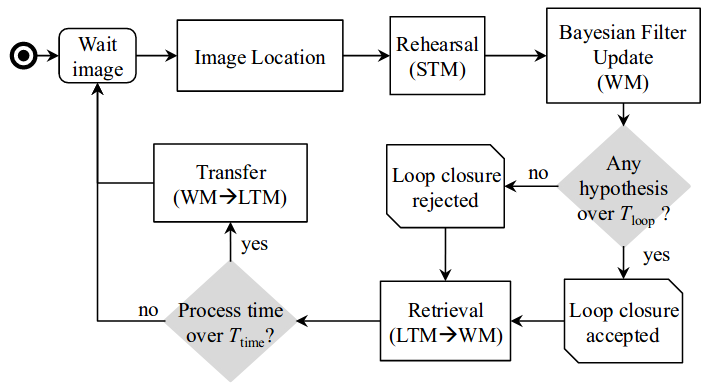
\includegraphics[scale=0.5]{img/rtabmap_loopclosure.png}
		\caption{Схема замыкания циклов в алгоритме RTAB-Map. Источник \cite{labbe2011memory}}
		\label{figureloopclosing}
	\end{figure}
	
	Данный алгоритм имеет следующие преимущества в сравнении с другими методами SLAM:
	\begin{enumerate}
		\item {Эффективная обработка данных с видеокамер и датчиков глубины в реальном времени}
		\item {Эффективное замыкание циклов}
		\item {Возможность работы в больших картах благодаря хранению долгосрочной памяти на жестком диске}
		\item {Высокая плотность построенной карты и возможность построения карты препятствий в формате Octomap}
		\item {Легкость использования в различных приложениях, а также большое количество настраиваемых параметров}
	\end{enumerate}
	Помимо преимуществ, алгоритм RTAB-Map обладает существенными недостатками:
	\begin{enumerate}
		\item {Невозможность работы в монокулярном режиме}
		\item {Потеря одометрии при отсутствии сопоставленных ориентиров}
		\item {Высокая ресурсоемкость из-за необходимости обработки трехмерных облаков точек и построения плотной карты}
	\end{enumerate}
	
	\subsection{RGBDSLAM\_v2}
	
	\begin{figure}
		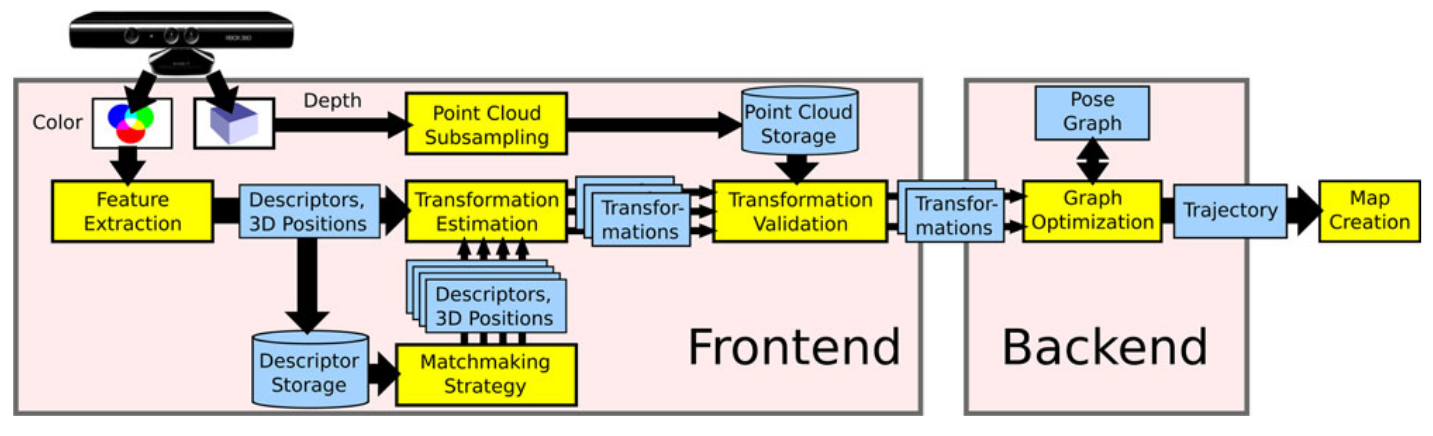
\includegraphics[width=1.0\textwidth]{img/rgbdslam_scheme.png}
		\caption{Общая схема алгоритма RGBDSLAM\_v2. Источник \cite{endres20133}}
		\label{figure_rgbdslam}
	\end{figure}
	
	Алгоритм RGBDSLAM\_v2 \cite{endres20133} также является популярным решением задачи одновременного картирования и локализации по данным с RGB-D камеры. Он был разработан примерно в то же время, что и описанный выше алгоритм RTAB-MAP, и основан на схожих принципах. Однако в деталях методов имеются существенные различия. Схема алгоритма RGBDSLAM\_v2 изображена на рисунке \ref{figure_rgbdslam}.
	
	Вычисление перемещения камеры в алгоритме RGBDSLAM\_v2 осуществляется по тем же принципам, что и в алгоритме RTAB-MAP - путем сопоставления особых точек на ключевых кадрах. Изображение с камеры добавляется в множество ключевых кадров, когда у него не будет совпадающих особых точек с предыдущим ключевым кадром. Для извлечения особых точек используются детекторы SIFT \cite{lowe2004distinctive}, SURF \cite{bay2006surf} или ORB \cite{rublee2011orb}. Сопоставления уточняются и фильтруются с помощью методов RANSAC \cite{brachmann2017dsac} и ICP \cite{chetverikov2005robust}. Преобразования, вычисленные по сопоставлениям особых точек, валидируются по картам глубин вероятностными методами.
	
	По ключевым кадрам и найденным преобразованиям строится граф поз. Вершинами в этом графе являются ключевые кадры, ребрами - вычисленные алгоритмом геометрические преобразования между кадрами. По данному графу проводится глобальная оптимизация с помощью библиотеки g2o \cite{grisetti2011g2o}.
	
	Метод замыкания циклов в алгоритме RGBDSLAM\_v2, так же, как и в RTAB-MAP, основан на вычислении преобразования по особым точкам между текущим кадром и похожими на него старыми ключевыми кадрами. Однако в алгоритме RGBDSLAM\_v2 используется более простой отбор кандидатов на ``похожесть''. По графу поз строится минимальное остовное дерево. В качестве кандидатов для рассмотрения выбираются $n$ предков текущего кадра в этом дереве, а также $k$ случайно выбранных ключевых кадров в части дерева, оставшейся после удаления этих $n$ предков, и еще $l$ ключевых кадров, случайно выбранных по всему графу. Для эффективного замыкания циклов на разных длинах траекторий необходимо использовать разные $n, k, l$.
	
	\begin{figure}
		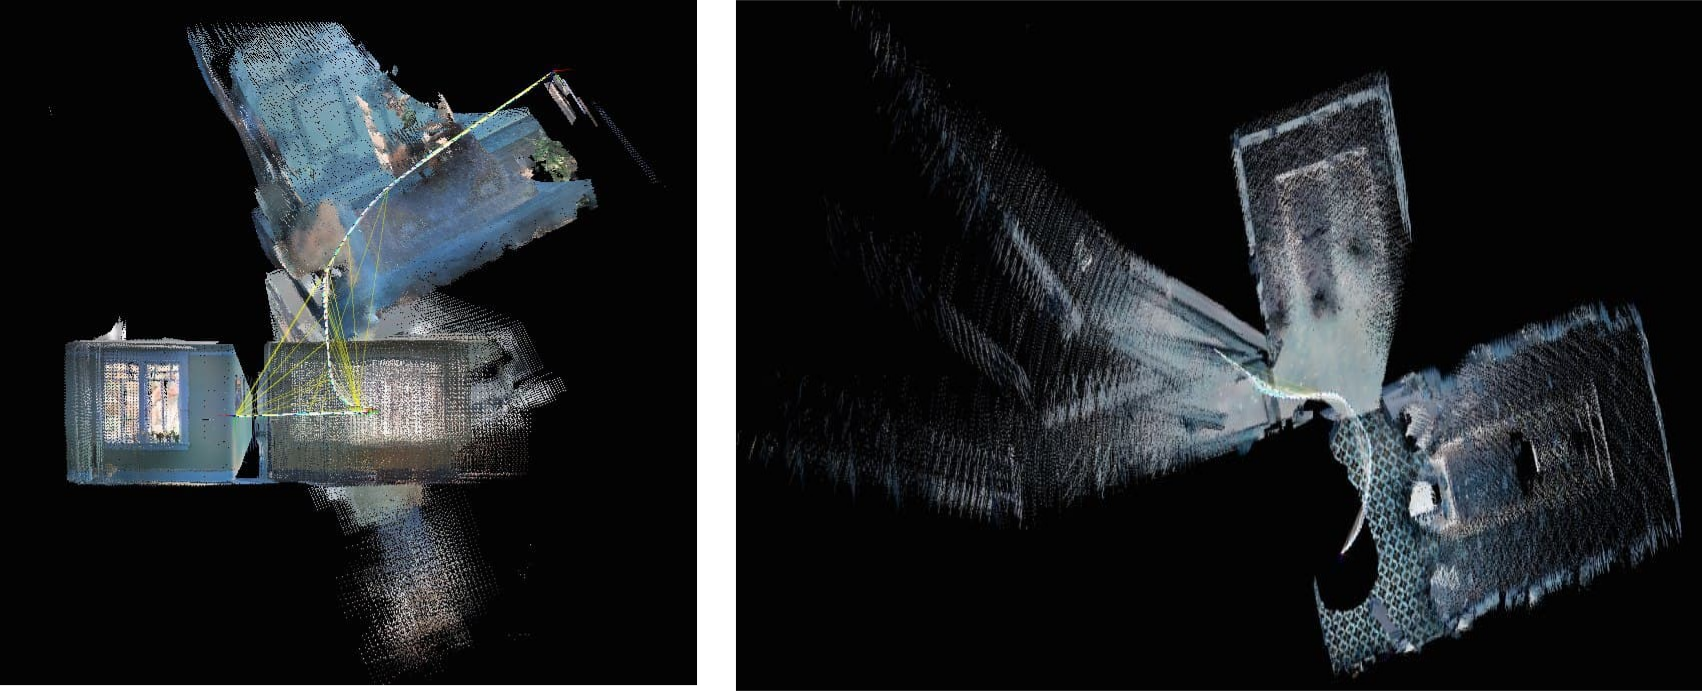
\includegraphics[width=1.0\textwidth]{img/rgbdslam_fails.png}
		\caption{Примеры некорректной работы алгоритма RGBDSLAM\_v2: ложное замыкание цикла (слева) и раздвоение коридора (справа)}
		\label{figure_rgbdslam_fails}
	\end{figure}
	
	Алгоритм RGBDSLAM\_v2 обладает высокой вычислительной эффективностью, однако эксперименты, проведенные в работе \cite{bokovoy2020map}, показали, что он обладает более низкой точностью по сравнению с алгоритмом RTAB-MAP. В частности, при резких поворотах робота RGBDSLAM\_v2 может найти ложные замыкания или построить карту с раздвоением коридора (см. рис. \ref{figure_rgbdslam_fails}).
	
	\section{Нейросетевые методы}
	
	В связи с бурным развитием вычислительной техники и нейронных сетей, в последние годы для решения задачи vSLAM также стали применяться методы, основанные на глубоком обучении. В подобных методах, как правило, вычисляются преобразования между позициями камеры с помощью сверточных нейронных сетей, также с помощью сверточных нейросетей вычисляются карты глубин по изображениям.
	
	Одним из наиболее известных нейросетевых методов картирования и локализации является CNN-SLAM \cite{tateno2017cnn}.	Как и в алгоритме LSD-SLAM \cite{engel2014lsd}, в CNN-SLAM из множества всех входящих кадров отбираются ключевые кадры. По ключевым кадрам строится граф позиций, который оптимизируется с помощью библиотеки g2o \cite{grisetti2011g2o}. По каждому кадру вычисляется преобразование между этим кадром и текущим ключевым кадром путем минимизации фотометрической ошибки.
	
	Метод CNN-SLAM принимает на вход видеопоток с камеры и по каждому изображению видеопотока вычисляет карту глубины с помощью полносверточной нейронной сети \cite{laina2016deeper}. Также вместе с картой глубины вычисляется карта неопределенности, которая показывает, насколько глубина объектов, изображенных на текущем кадре, соотносится с глубинами этих объектов на других кадрах. Глубина каждого кадра оптимизируется исходя из карты неопределенности и глубины текущего ключевого кадра.
	 
	Помимо карты глубины, по каждому кадру входящего видеопотока с помощью нейросети выполняется семантическая сегментация. По картам глубин и картам сегментации с помощью глобальной сегментационной модели (GSM) \cite{tateno2015real} строится итоговая карта окружающей местности.
	
	Эксперименты на датасетах TUM \cite{sturm2012benchmark} и ICL-NUIM \cite{handa2014benchmark} показали, что по точности определения местоположения алгоритм CNN-SLAM более чем в два раза превосходит классический метод LSD-SLAM \cite{engel2014lsd}. Однако качество метода CNN-SLAM, как и любого метода, использующего предобученные нейросети, сильно зависит от качества обучающей выборки.
	
	Одним из наиболее известных недавних нейросетевых методов vSLAM является Active Neural SLAM \cite{chaplot2020learning}. Данный метод решает задачу vSLAM в контексте более глобальной задачи - исследование неизвестной местности (Exploration). Помимо картирования и локализации, алгоритм выполняет постановку цели для исследования и планирование траектории.
	
	\begin{figure}
		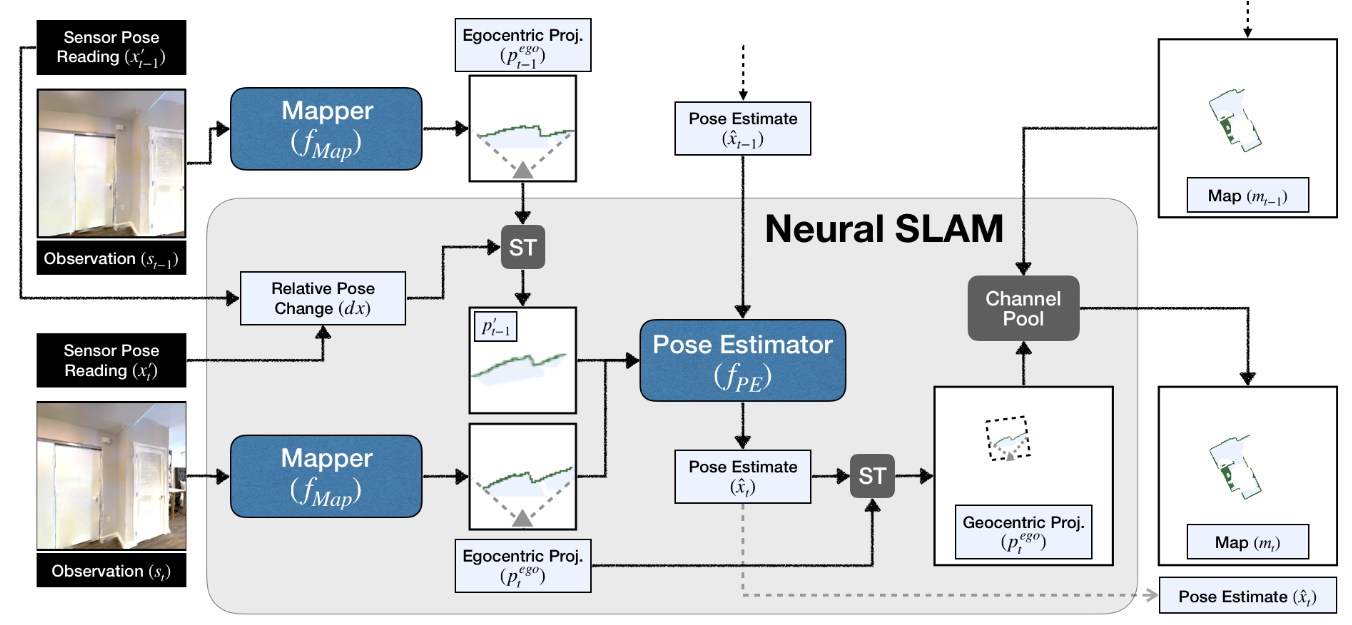
\includegraphics[width=1.0\textwidth]{img/ans_scheme.png}
		\caption{Схема метода Active Neural SLAM. Источник \cite{chaplot2020learning}}
		\label{figure_active_neural_slam}
	\end{figure}
		
	Метод Active Neural SLAM принимает на вход видеопоток с камеры и данные одометрии с сенсоров робота. На выходе получается двумерная карта местности и траектория перемещения робота. В отличие от метода CNN-SLAM, где карта строится по предсказанным нейросетью глубинам с помощью различных методов оптимизации, в методе Active Neural SLAM локальные карты предсказываются непосредственно нейросетью по каждому изображению видеопотока. Перемещение робота также предсказывается нейросетью по локальным картам входящим данным одометрии (как правило, сильно зашумленным). Схема алгоритма Active Neural SLAM изображена на рисунке \ref{figure_active_neural_slam}.
	
	Эксперименты, проведенные на датасете Gibson \cite{xia2018gibson}, показали, что метод Active Neural SLAM способен исследовать в среднем 95\% помещения, решая задачу vSLAM совместно с задачей планирования маршрутов и исследования неизвестной местности. Однако оценка качества построения карты и вычисления траектории в работе \cite{chaplot2020learning} не производилась.
	
	\section{Выводы}
	
	В данной главе были рассмотрены классические и нейросетевые методы решения задачи vSLAM. Среди классических методов были рассмотрены следующие:
	
	\begin{enumerate}
		\item ORB-SLAM - метод, основанный на сопоставлении особых точек на изображениях
		\item LSD-SLAM - метод, основанный на вычислении геометрических преобразований путем минимизации фотометрической ошибки
		\item RTAB-MAP - метод, принимающий на вход данные со стереокамеры или RGB-D камеры, обладающий эффективным замыканием циклов
		\item RGBDSLAM - метод, принимающий на вход данные с RGB-D камеры, с более простым замыканием циклов по сравнению с RTAB-MAP
	\end{enumerate}

	Алгоритм ORB-SLAM обладает высокой вычислительной эффективностью, однако строит разреженную карту местности, не пригодную для планирования маршрутов. Метод LSD-SLAM строит довольно плотную карту, однако он более требователен к вычислительным ресурсам и имеет в среднем более низкую точность. Методы RTAB-MAP и RGBDSLAM строят плотную карту и имеют довольно высокую точность, однако они требуют на вход данные со стереокамеры или RGBD-камеры. Для их работы по данным с единственной камеры может применяться восстановление глубин изображений с помощью нейронных сетей.
	
	Помимо классических методов, были также рассмотрены нейросетевые методы картирования и локализации:
	
	\begin{enumerate}
		\item CNN-SLAM - построение карты по предсказанным нейросетью глубинам и картам сегментации с помощью глобальных моделей
		\item Active Neural SLAM - построение карты и вычисление траектории с помощью нейросетей непосредственно
	\end{enumerate}

	На некоторых коллекциях данных методы CNN-SLAM и Active Neural SLAM имеют более высокое качество по сравнению с классическими методами. Однако их применение на реальных роботах затруднено, поскольку данные методы требуют наличие графического ускорителя на борту, и качество их работы напрямую зависит от выборки, на которой производилось обучение нейросетей.
	
	В данной работе был выбран алгоритм RTAB-MAP, поскольку он строит плотную трехмерную карту местности и не требователен к вычислительным ресурсам. Для применения алгоритма на данных с единственной видеокамеры используется восстановление карт глубин с помощью полносверточных нейронных сетей с легкой архитектурой, способных работать с высокой скоростью в условиях ограниченных вычислительных ресурсов.
		
	%-----------------------------------------------------------------------------------------------------------------------
	% AUXILIARY TASKS
	%-----------------------------------------------------------------------------------------------------------------------
	
	\chapter{Вспомогательные задачи для vSLAM}
	
	\section{Восстановление глубины по видеопотоку}
	
	Классические методы решения задачи vSLAM по данным с монокулярной камеры \cite{mur2015orb} \cite{engel2014lsd}, описанные в предыдущей главе, выдают разреженную карту, непригодную для планирования маршрутов. Построение плотной карты возможно при наличии информации о глубине изображений, например, при помощи методов \cite{labbe2011memory}, \cite{endres20133}. Таким образом, для построения плотной карты окружающей местности по данным с единственной видеокамеры необходимо решить задачу восстановления глубины изображений. Схема метода vSLAM с использованием восстановления глубины изображений показана на рисунке \ref{figure_our_slam_pipeline}.
	
	\begin{figure}
		\centering
		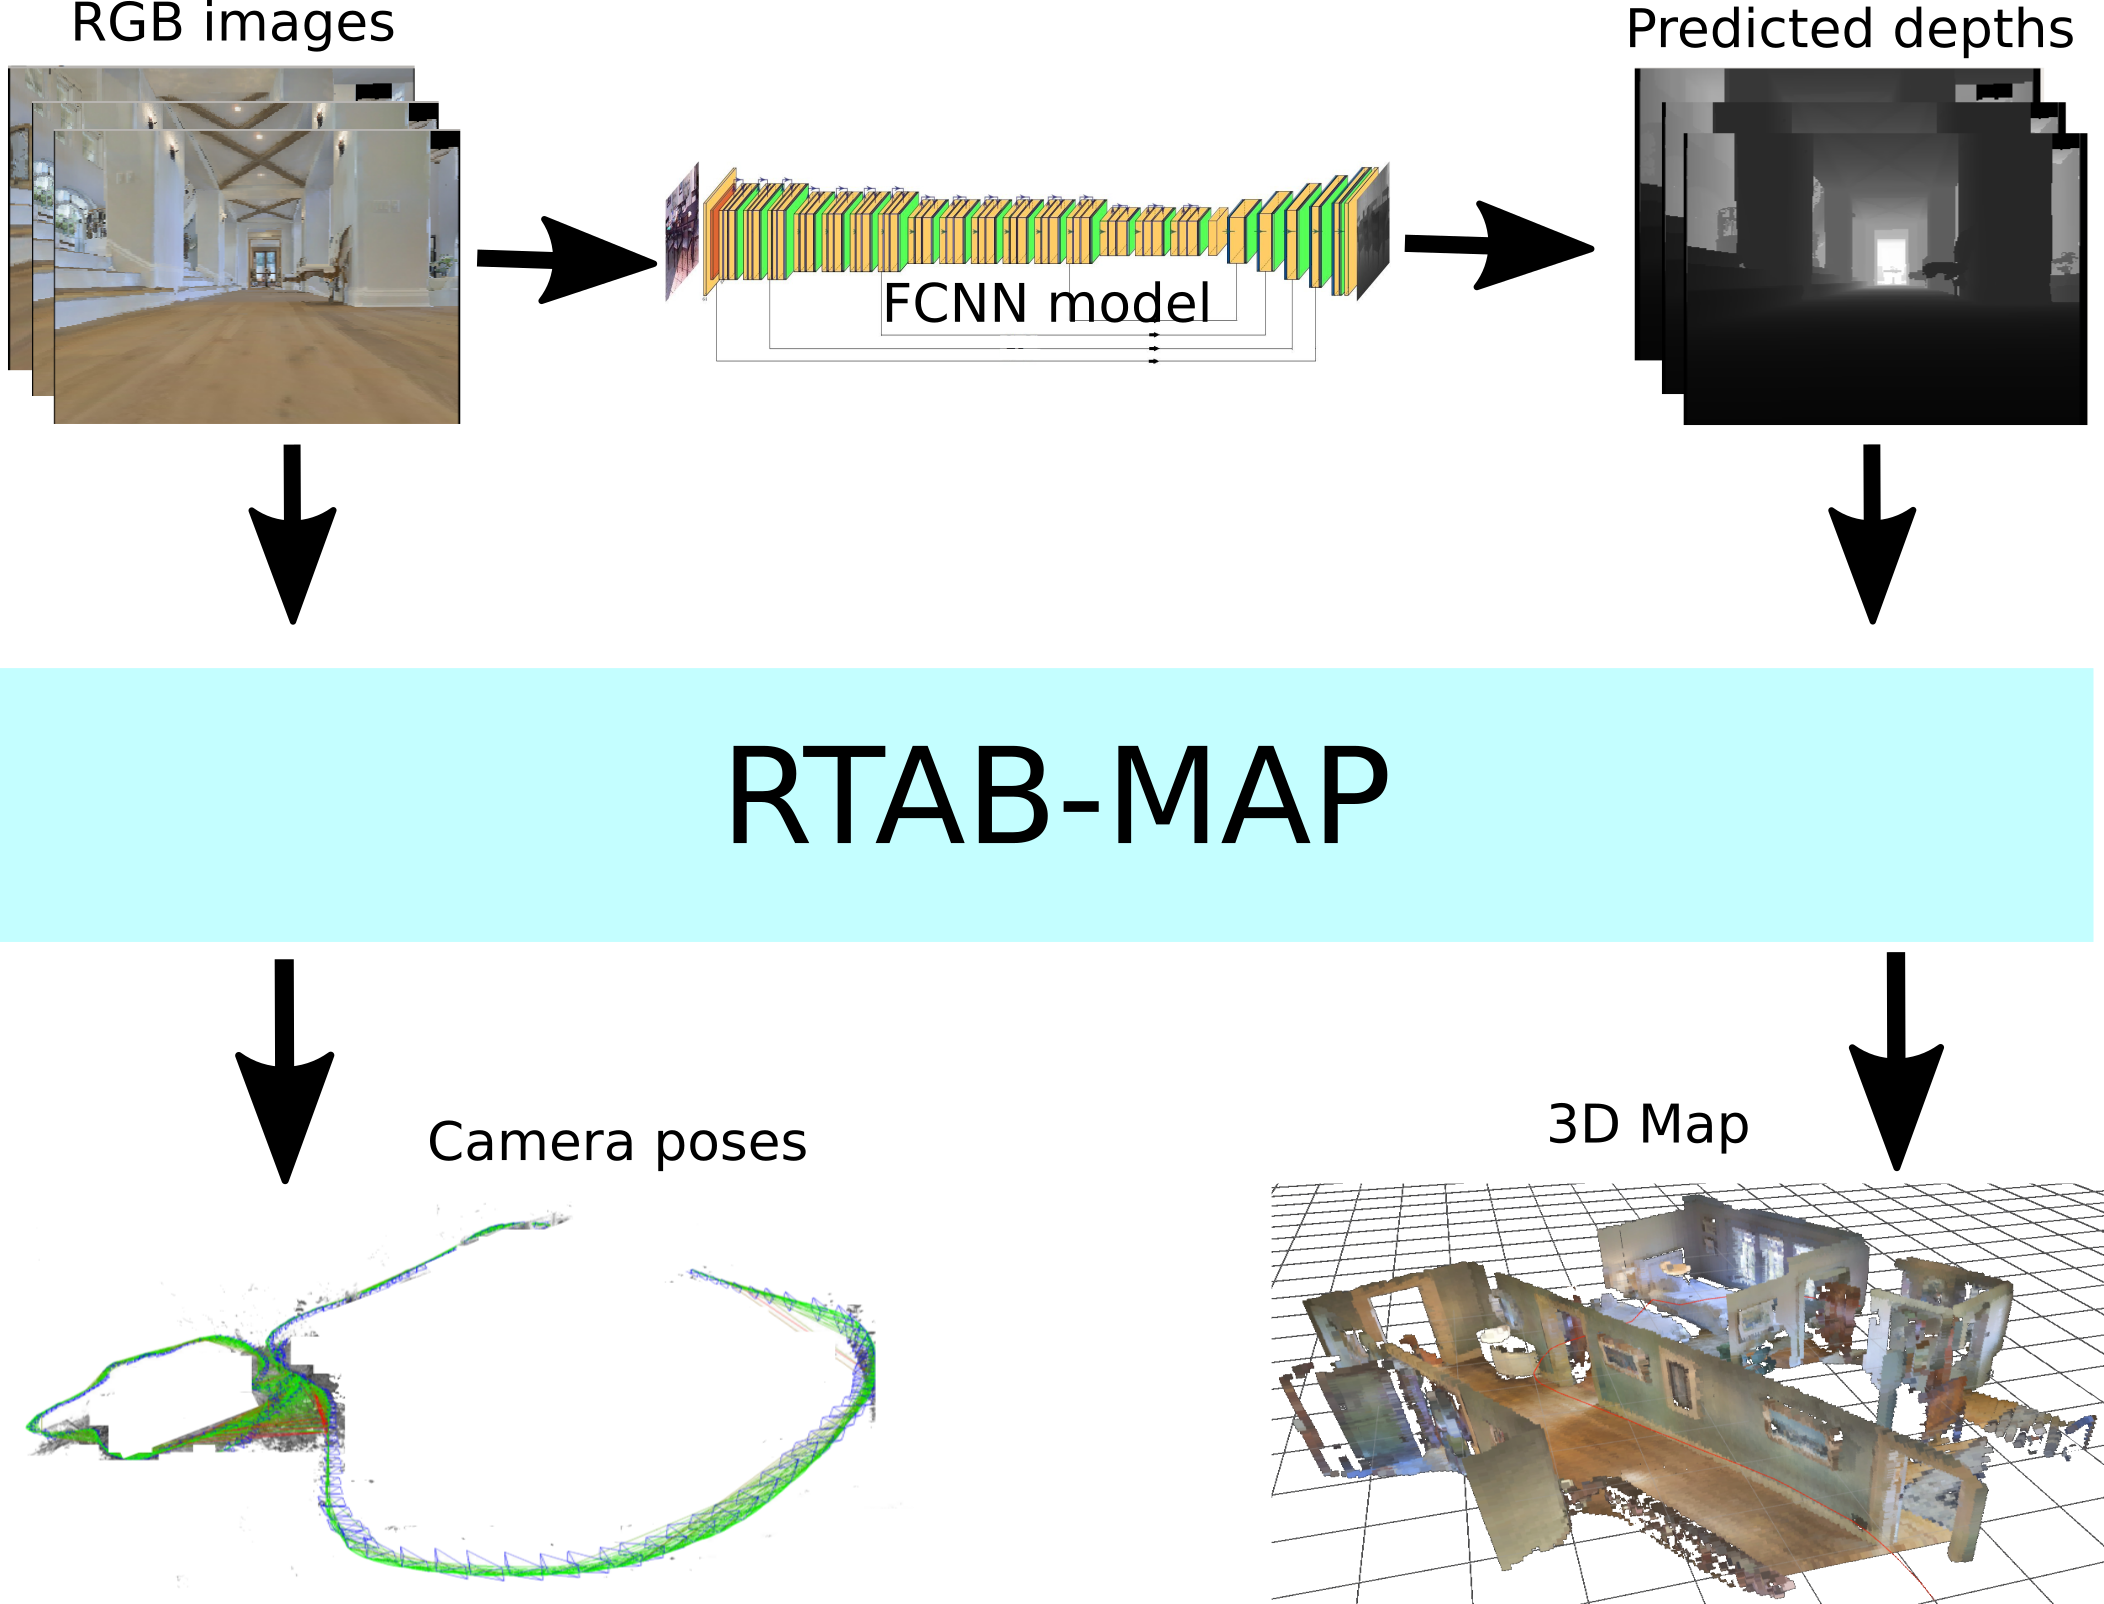
\includegraphics[width=0.7\textwidth]{img/slam_scheme.png}
		\caption{Схема представленного в данной работе метода vSLAM. По изображениям с камеры при помощи нейронной сети вычисляются карты глубин, которые вместе с изображениями подаются на вход алгоритму RTAB-MAP. Алгоритм RTAB-MAP выдает плотную трехмерную карту окружающей местности и траекторию перемещения камеры}
		\label{figure_our_slam_pipeline}
	\end{figure}
	
	В настоящее время задача восстановления глубины изображений решается, как правило, с помощью глубоких нейронных сетей. Нейросети, предсказывающие глубину изображений по видеопотоку, делятся на два типа. Первые принимают на вход одиночное изображение, не используя информацию о контексте из видео. Вторые предсказывают глубину изображений с использованием информации об изменении положений объектов на кадрах видеопотока. Ниже рассмотрены обе группы нейросетевых методов восстановления глубины.
	
	\subsection{Восстановление глубины по одиночным изображениям}
	
	В настоящее время существует большое количество нейросетевых архитектур для восстановления глубины по одиночным изображениям. Как правило, такие нейросети состоят из сверточного энкодера и декодера, состоящего из нескольких блоков, в которых используются слои свертки и повышения дискретизации (Upsampling).
	
	Одной из наиболее известный нейросетей восстановления глубины является FCRN \cite{laina2016deeper}. Архитектура данной сети состоит из энкодера и декодера. В качестве энкодера выбрана широко известная сеть ResNet \cite{he2016deep}, содержащая 50 сверточных слоев. В качестве декодера используется 5 блоков Up-Convolution или Up-Projection (см. рис. \ref{figure_upconv_upproj}).
	
	\begin{figure}
		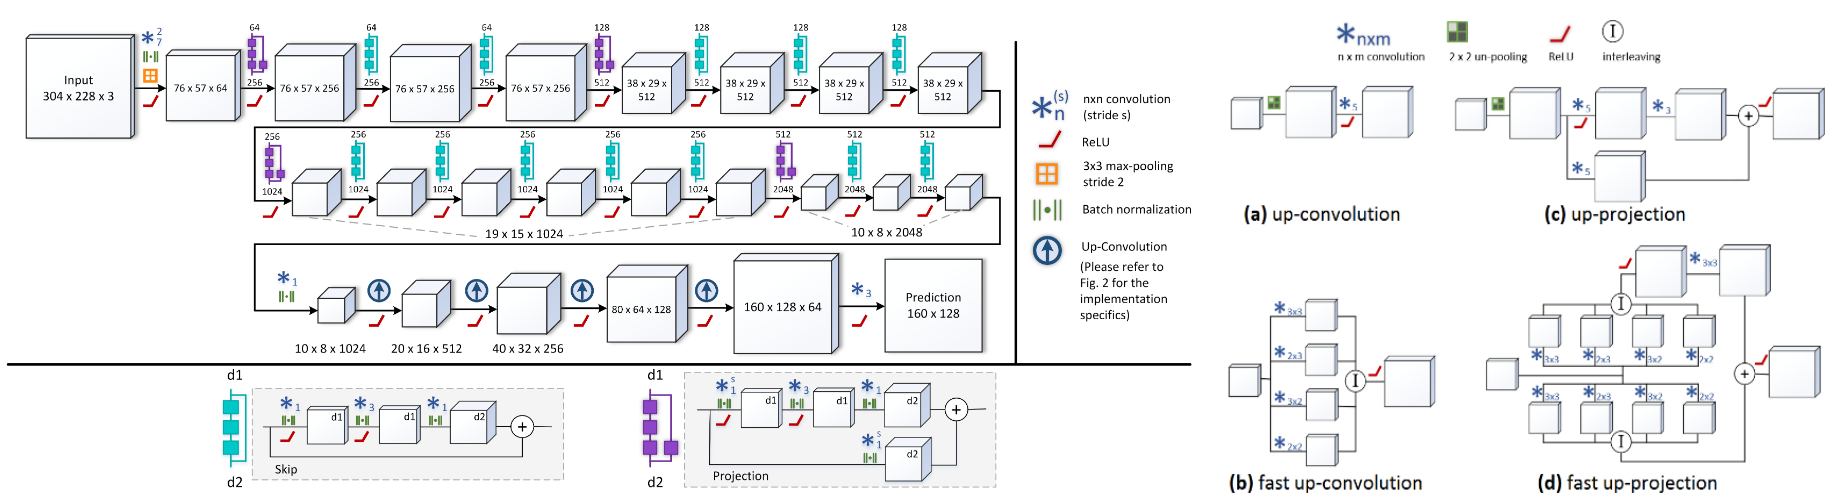
\includegraphics[width=1.0\textwidth]{img/fcrn_scheme_full.png}
		\caption{Схема архитектуры FCRN (слева) и различных блоков декодера - Up-Projection и Up-Convolution (справа). Источник \cite{laina2016deeper}}
		\label{figure_upconv_upproj}
	\end{figure}

	Обучение сети FCRN производилось на датасете NYU Depth v2 \cite{silberman2012indoor}. Исследовались разные функции потерь - стандартная функция MSE, а также функции Huber и BerHu \cite{owen2007robust} \cite{zwald2012berhu}, являющиеся комбинацией квадратичной и линейной ошибки. Наилучший результат показала архитектура с декодером Up-Projection, обученная с функцией потерь BerHu. Относительная ошибка этой архитектуры на валидационной выборке NYU Depth v2 составила 0.127. Была также измерена скорость работы данной архитектуры на видеокарте GTX Titan. Она составила 78 мс на одно изображение, или 13 кадров в секунду, что недостаточно для работы в реальном времени (для обработки всех кадров стандартного видеопотока необходима скорость не менее 30 кадров в секунду).
	
	В 2020 году была предложена нейросетевая архитектура восстановления глубины с более высокой скоростью и качеством работы \cite{huynh2020guiding}. В этой архитектуре предсказание глубины уточняется с помощью механизма внимания, установленного между энкодером и декодером. Механизм внимания предсказывает, насколько глубина одного участка изображения может быть полезна для предсказания глубины другого участка, формируя карты внимания глубины (depth-attention maps). Для построения истинных карт внимания, необходимых для обучения сети, по изображенному на кадре участку сцены вычисляется несколько плоскостей. Значением внимания глубины одного пикселя для другого является максимальная сумма расстояний точек, спроецированных в эти пиксели, до плоскостей. Такой метод обосновывается тем, что у точек, расположенных в одной плоскости, легко вычислить глубину с помощью геометрических преобразований, если известна точная глубина хотя бы одной из этих точек.
	
	С помощью вышеописанной архитектуры и механизма внимания была достигнута относительная ошибка 0.108 на датасете NYU Depth v2. Скорость работы данной архитектуры на видеокарте GTX 1080 составила 218 кадров в секунду. Однако на бортовых вычислителях робототехнических систем, не обладающих мощными видеокартами, скорость работы нейросети будет значительно меньше. Точно измерить скорость работы описанной нейросети на бортовых вычислителях не удалось, поскольку исходный код описанной архитектуры на момент написания данной работы предоставлен не был.
	
	\begin{figure}
		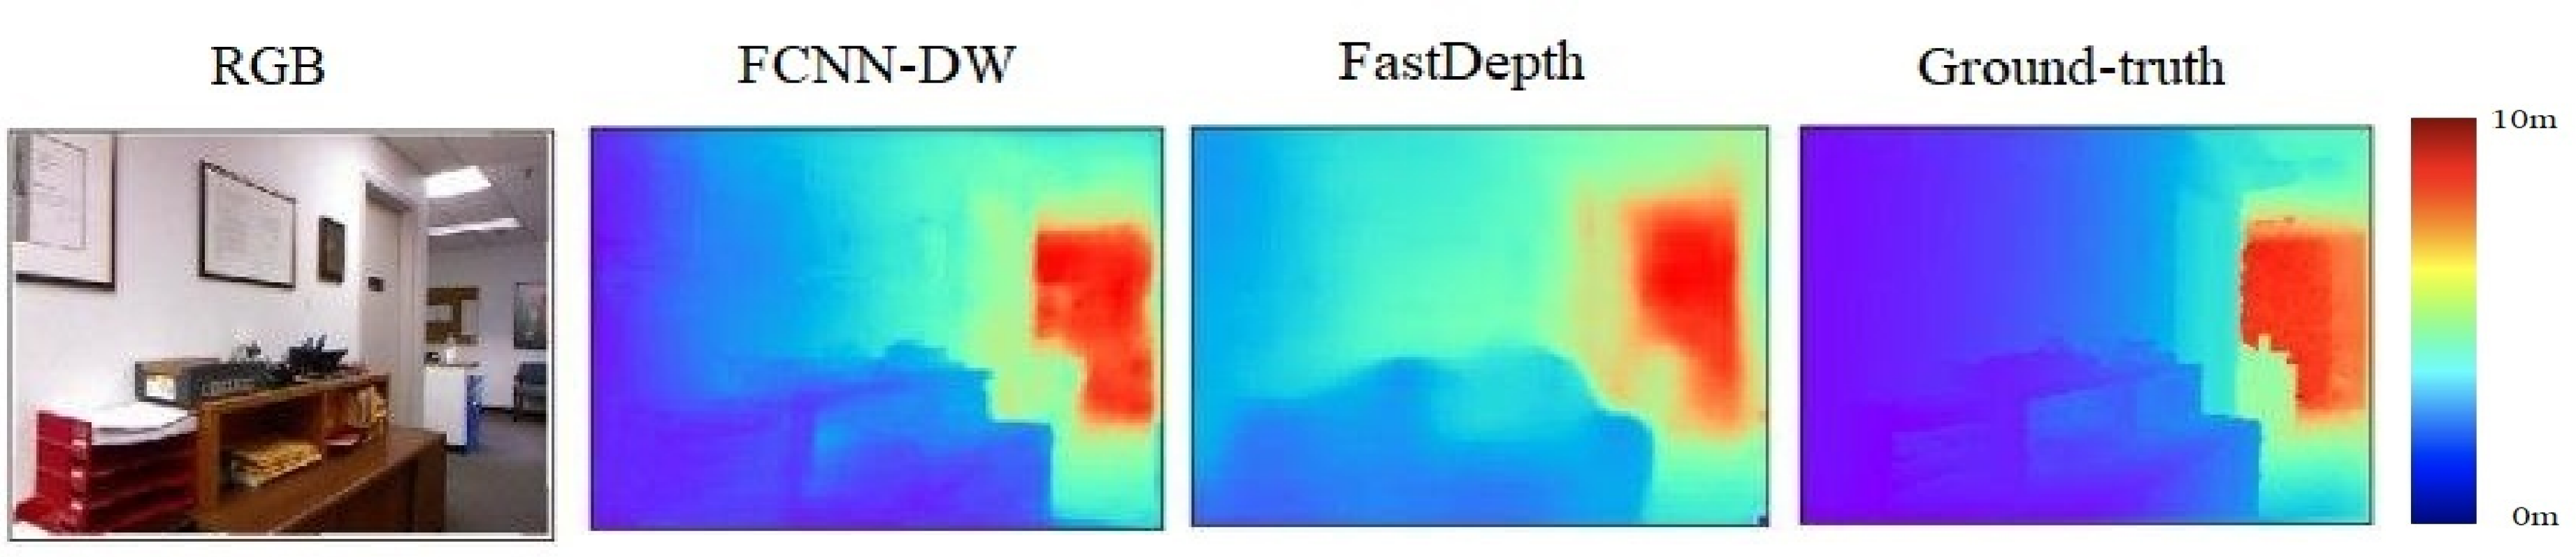
\includegraphics[width=1.0\textwidth]{img/fcnn_depths_nyu.png}
		\caption{Примеры глубин, предсказанных нейросетью FastDepth (справа), в сравнении с глубинами, предсказанными нейросетями из данной работы}
		\label{figure_fastdepth_preidctions}
	\end{figure}
	
	В работе \cite{wofk2019fastdepth} описана архитектура FastDepth, пригодная для работы в реальном времени даже на маломощных вычислительных устройствах. С помощью различных технических и архитектурных оптимизаций авторам работы удалось добиться скорости восстановления глубины 175 кадров в секунду на встраиваемом компьютере NVidia Jetson TX2, который широко используется в различных робототехнических системах. Ошибка восстановления глубины на NYU Depth v2 при этом составила 0.158 - почти в полтора раза выше, чем у архитектуры из работы \cite{huynh2020guiding}. Контуры объектов на предсказанных картах глубины также получились размытыми (см. рис. \ref{figure_fastdepth_preidctions}), что может негативно сказаться на качестве карты при применении предсказанных глубин в задаче vSLAM.
	
	В данной работе с учетом преимуществ и недостатков всех вышеописанных методов была разработана новая нейросетевая архитектура для достижения баланса между скоростью и качеством восстановления глубины. В основе разработанной архитектуры лежит классическая схема энкодер-декодер. В качестве энкодера выбрана сеть ResNet с 50 слоями, как и в архитектуре FCRN. В качестве декодера была выбрана серия сверток depthwise convolution, как и в архитектуре FastDepth. Также для повышения качества работы и четкости контуров были добавлены проекции из энкодера в декодер (shortcuts). С помощью предложенной архитектуры удалось достичь приемлемого качества восстановления глубины (относительная ошибка 0.170 на NYU Depth v2) и вместе с тем приемлемой скорости работы (24 кадра в секунду на NVidia Jetson TX2). Примеры глубин, предсказанных разработанной нейросетью, показаны на рисунке \ref{figure_fastdepth_preidctions} посередине.
	
	\subsection{Восстановление глубины с извлечением информации из видеопотока}
	
	При наличии видеопотока можно получить дополнительную информацию о глубине изображений из перемещения объектов на кадрах. Например, в методе LSD-SLAM \cite{engel2014lsd} карты глубин изображений вычисляются с использованием преобразований подобия, задающих перемещение камеры от кадра к кадру и вычисляемых путем минимизации фотометрической ошибки. С помощью глубоких нейронных сетей также можно извлекать временную информацию из видеопотока, тем самым уточняя карты глубин каждого изображения.
	
	\begin{figure}
		\centering
		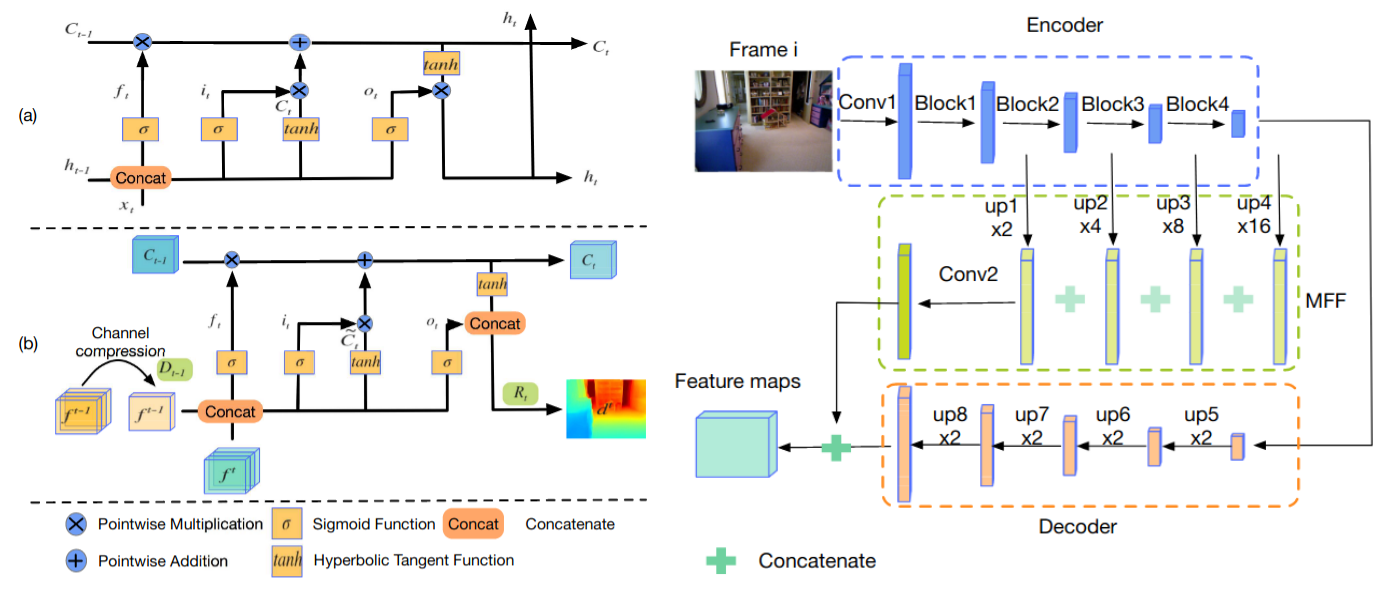
\includegraphics[width=0.9\textwidth]{img/st_clstm_scheme.png}
		\caption{Схема архитектуры ST-CLSTM: часть, кодирующая пространственные признаки (слева), и модуль Conv-LSTM (справа). Источник \cite{zhang2019exploiting}}
		\label{figure_conv_lstm}
	\end{figure}
	
	В работе \cite{zhang2019exploiting} описана архитектура нейронной сети ST-CLSTM, в которой временная информация извлекается из видеопотока с помощью сверточно-рекуррентных блоков ConvLSTM. Модуль ConvLSTM представляет собой комбинацию слоев, используемую в традиционном модуле LSTM \cite{greff2016lstm}, в которой полносвязные слои заменены на сверточные.
	
	Архитектура ST-CLSTM состоит из двух частей. Её схема изображена на рисунке \ref{figure_conv_lstm}. Первая часть имеет схему энкодер-декодер и по входящему изображению вычисляет набор пространственных признаков. В качестве энкодера используется сеть ResNet-18 \cite{he2016deep}. Декодер представляет собой четыре блока, состоящих из последовательного повышения дискретизации и двух параллельных сверток. Для повышения информативности вычисляемых признаков в архитектуру первой части встроен также модуль слияния признаков с несколькими масштабами (Multi-scale feature fusion, MFF). Модуль MFF представляет собой конкатенацию выходов четырех блоков энкодера, приведенных к размеру исходного изображения с помощью слоев повышения дискретизации (Upsampling). Данная конкатенация преобразуется с помощью сверточного слоя и стыкуется с выходом декодера, в результате чего получается карта пространственных признаков.
	
	Вторая часть архитектуры ST-CLSTM состоит из блока ConvLSTM и двух сверточных слоев. Слои блока ConvLSTM используют информацию, извлеченную из карт пространственных признаков предыдущих изображений. Сверточные слои преобразуют данную информацию в карту глубины.
	
	Для обучения сети ST-CLSTM использовалась комбинация пространственной и временной функции потерь. Пространственная функция потерь представляла собой среднюю логарифмическую ошибку между предсказанной и истинной глубиной. Для эффективного обучения временной составляющей сети ST-CLSTM применялся генеративно-состязательный подход. В качестве генератора выступала непосредственно сеть ST-CLSTM, а в качестве дискриминатора - трехмерная сверточная нейронная сеть, принимающая на вход последовательность карт глубин и предсказывающая происхождение этих глубин (истинные или предсказанные нейросетью-генератором).
	
	Эксперименты, проведенные на датасете NYU Depth v2 \cite{silberman2012indoor}, показали, что с помощью архитектуры ST-CLSTM удалось добиться довольно высокого качества восстановления глубины. Относительная ошибка составила 0.132. В ходе экспериментов была также измерена скорость обработки одного изображения на видеокарте GTX 1080Ti. Скорость работы оказалась равной 33 кадрам в секунду, что достаточно для обработки видеопотока в реальном времени. Однако на менее мощной видеокарте, в частности, на бортовых вычислителях большинства робототехнических систем, данная архитектура будет работать значительно медленнее, что затруднит ее использование в реальном времени. Например, скорость работы на встраиваемом компьютере NVidia Jetson TX2 составила менее 10 кадров в секунду.
	
	В работе \cite{luo2020consistent} для предсказания глубины изображений используется традиционная полносверточная нейросеть, а предсказанные нейросетью глубины дополнительно уточняются с помощью оптического потока и метода COLMAP \cite{schonberger2016structure}. Оптический поток вычисляется нейронной сетью FlowNet2 \cite{ilg2017flownet}.
	
	С помощью вычисленного оптического потока нейросеть восстановления глубины может дообучаться на конкретном видео без данных об истинных глубинах изображений. По предсказанным нейросетью глубинам и перемещениях пикселей изображений (оптического потока) вычисляется временная консистентность, которая служит в данном случае функцией потерь при обучении.
	
	Коррекция предсказанных глубин методом COLMAP позволила существенно повысить качество восстановления глубины в тех случаях, когда тестовая выборка значительно отличается от обучающей. Так, на датасете ScanNet \cite{dai2017scannet} относительная ошибка предсказания глубины составила 0.073 (против 0.208 у полносверточной нейронной сети без коррекции). Однако данный подход малопригоден для применения в реальном времени на борту робота - нейросеть FlowNet, вычисляющая оптический поток, обрабатывает одну пару кадров более 100 мс на видеокарте компьютера NVidia Jetson TX2; а также метод COLMAP потребляет значительную часть ресурсов процессора, что затрудняет работу алгоритмов SLAM.
	
	В работах \cite{zhou2017unsupervised}, \cite{yang2020d3vo}, \cite{teed2018deepv2d} совместно с задачей восстановления глубины решается также задача визуальной одометрии - вычисления перемещения камеры по видеоданным с нее. Для вычисления карт глубин и перемещения камеры используются отдельные нейронные сети, которые обучаются совместно с использованием общей функции потерь, основанной на пространственно-временной консистентности. Таким образом, возможно обучение нейросетей при отсутствии данных об истинной глубине изображений, на неразмеченном видеопотоке.
	
	Совместное использование нейросетей глубины и позиции позволило достичь очень низкой ошибки восстановления глубины. Так, в работе \cite{teed2018deepv2d} относительная ошибка на датасете NYU Depth v2 \cite{silberman2012indoor} составила 0.061 (по сравнению с ошибкой в 0.106 у классических полносверточных нейросетей). Однако параллельная работа двух нейронных сетей в реальном времени на бортовом вычислителе затруднительна. Так, в работе \cite{teed2018deepv2d} время обработки одного кадра составляет 690 мс (при том, что в стандартном видеопотоке кадры приходят каждые 33 мс).
	
	\subsection{Выводы}
	
	Восстановление глубины изображений дает возможность строить плотную карту местности по данным с единственной видеокамеры с помощью методов vSLAM. В данной главе приведен обзор основных методов восстановления глубины по изображениям. Методы, использующие в качестве входных данных одиночное изображение (\cite{laina2016deeper}, \cite{wofk2019fastdepth}) обладают достаточно высокой скоростью работы для обработки стандартного видеопотока в реальном времени, однако имеют довольно низкое качество (относительная ошибка порядка 13-17\%). Методы, принимающие во внимание информацию о перемещении между кадрами (\cite{zhang2019exploiting} \cite{luo2020consistent} \cite{teed2018deepv2d}), имеют значительно более высокое качество (относительная ошибка восстановления глубины порядка 6-10\%), однако обладают низкой скоростью работы, что затрудняет их применение на борту робототехнической системы в реальном времени.
	
	В данной работе для решения задачи VSLAM была выбрана полносверточная нейронная сеть, принимающая на вход одиночные изображения. Архитектура нейронной сети была оптимизирована для работы в реальном времени на встраиваемом компьютере NVidia Jetson TX2, который может применяться в качестве бортового вычислителя на малых робототехнических системах. Подробное описание данной архитектуры приведено в главе \ref{chapter_our_slam}.
	
	%------------------------------------------------------------------------------------------------------------------------------
	% OUR SLAM
	%------------------------------------------------------------------------------------------------------------------------------
	
	\chapter{Одновременное картирование и локализация с использованием вспомогательных методов}
	\label{chapter_our_slam}
	
	\section{Описание метода}
	
	В данной работе представлен алгоритм одновременного картирования и локализации по видеопотоку с единственной камеры, основанный на восстановлении карт глубин изображений. По изображениям, поступающим с видеокамеры, вычисляются карты глубин с помощью полносверточной нейронной сети. По изображениям и предсказанным картам глубин осуществляется картирование и локализация с помощью метода RTAB-Map, описанного в разделе \ref{section_rtabmap}. Схема алгоритма представлена на рисунке \ref{figure_our_slam_pipeline}.
	
	\begin{figure}
		\centering
		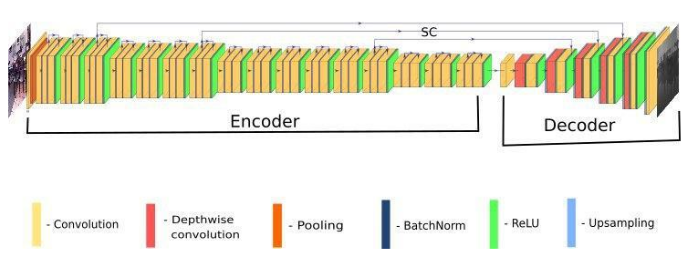
\includegraphics[width=0.9\textwidth]{img/fcnn_scheme.png}
		\caption{Схема нейронной сети восстановления глубины}
		\label{figure_our_fcnn}
	\end{figure}
	
	Нейросеть, используемая для восстановления глубины, имеет полносверточную архитектуру, состоящую из энкодера и декодера. Сеть принимает на вход трехканальное цветное изображение размера 320х240 и выдает карту глубины такого же размера. В качестве энкодера используется сеть ResNet-50 \cite{he2016deep} без полносвязных слоев, предобученная на датасете MS Coco \cite{lin2014microsoft}. На выходе энкодера получается карта высокоуровневых признаков размерности 10х8х2048. Декодер состоит из пяти блоков, каждый из которых повышает пространственную размерность в два раза. Каждый блок состоит из слоя повышения дискретизации (Upsampling), свертки с ядром 1х1 (pointwise convolution) и поканальной свертки (depthwise convolution) с ядром 3х3. Схема архитектуры нейросети представлена на рисунке \ref{figure_our_fcnn}.
	
	Обучение нейросети восстановления глубины проводилось на датасете NYU Depth v2 \cite{silberman2012indoor}. Датасет содержит 464 видеопоследовательности, снятые в разных помещениях с размеченными картами глубин. Суммарно во всех последовательностях содержится более 400000 пар изображение-глубина. Для обучения была отобрана выборка из 10\% (порядка 40000) изображений датасета. Из них около 30000 изображений составляла обучающая выборка и около 10000 - валидационная. В обущчающей и валидационной выборке использовались изображения из разных сцен.
	
	Оптимизация параметров проводилась методом Adam \cite{kingma2014adam} с параметрами $beta_1 = 0.9, beta_2 = 0.999$ в течение 30 эпох. В качестве функции потерь использовалась комбинация среднеквадратичной и относительной квадратичной ошибки между истинной и предсказанной глубиной:
	
	\begin{equation}
		L(D, \widehat{D}) = \frac{1}{H \cdot W} (\sum\limits_{i,j} (D_{i,j} - \widehat{D}_{i,j})^2 + \alpha \sum\limits_{i,j} (\frac{D_{i,j} - \widehat{D}_{i,j}}{D_{i,j}})^2),
	\end{equation}
	
	где $D_{i,j}, i=1,\dots,H; j=1,\dots,W$ - истинные значения глубин, а $\widehat{D}_{i,j}, i=1,\dots,H; j=1,\dots,W$ - предсказанные значения глубин.
	
	\begin{table}[h]
		\caption{Оценка качества восстановления глубины и сравнительный анализ различных нейросетей}
		\label{table_nyu_results}
		\begin{center}
			\resizebox{1.0\textwidth}{!}{
				\begin{tabular}{|c||c c||c c c||c|}
					\hline
					\multirow{2}{*}{\textbf{Архитектура}} & \multicolumn{2}{c||}{\textbf{NYU Dataset v2}} & \multicolumn{3}{c||}{\textbf{RealSense}} & \multirow{2}{*}{\textbf{FPS}} \\
					\cline{2-6}
					& \textbf{RMSE} & \textbf{REL} & RMSE & REL & $\delta^1$ & \\
					\hline
					\hline
					FastDepth \cite{wofk2019fastdepth} & \textbf{0.594} & 0.170 & 1.315 & 0.292 & 0.467 & \textbf{55} \\
					
					FCNN-nonbt (ours) \cite{bokovoy2019real} & 0.647 & 0.173 & \textbf{0.936} & \textbf{0.202} & \textbf{0.608} & 16\\
					
					FCNN-DW (ours) & 0.696 & \textbf{0.158} & 1.179 & 0.257 & 0.441 & 24\\
					\hline
			\end{tabular}}
		\end{center}
	\end{table}
	
	После обучения была проведена оценка качества нейросети на официальной тестовой выборке датасета NYU Depth v2, содержащей 1449 изображений с высокоточной глубиной с качественной пост-обработкой. Также для проверки устойчивости нейросети к изменениям выборки была проведена оценка качества на наборе данных, собранных с RGB-D камеры Intel Realsense. Набор содержал приблизительно 9500 пар изображение-глубина.
	
	Для оценки качества вычислялись три основные метрики: среднеквадратичная ошибка (RMSE), относительная ошибка (REL), и также метрика $\delta_1$ - доля пикселей, на которых относительная ошибка глубины не превысила 0.25. Помимо метрик качества, также была измерена скорость обработки изображений на бортовом компьютере NVidia Jetson TX2. Результаты сравнения представлены в таблице \ref{table_nyu_results}.
	
	Эксперименты показали, что представленная в данной работе нейросеть имеет приемлемое качество восстановления глубины, сравнимое с другими современными архитектурами, и при этом обладает достаточной эффективностью для работы в реальном времени на встраиваемом компьютере (при скорости в 24 кадра в секунду сеть способна обрабатывать почти каждый кадр входящего видеопотока). Данная сеть показывает схожие значения метрик качества с архитектурой FastDepth \cite{wofk2019fastdepth}, однако предсказанные глубины у нее получаются значительно более четкими (см. рис. \ref{figure_fastdepth_preidctions}). Также эксперименты показали, что данная нейросеть обладает более высокой обобщающей способностью, чем FastDepth (качество восстановления глубины на данных с RealSense оказалось лучше по всем метрикам).
	
	Помимо оценки качества восстановления глубины, была также проведена оценка качества работы метода vSLAM с разными нейросетевыми архитектурами восстановления глубины. Результаты оценки качества vSLAM описаны ниже.
	
	\section{Программно-аппаратное обеспечение}
	
	Архитектура нейросети была построена с использованием библиотеки глубинного обучения TensorFlow и ее расширения Keras. Программный код построения архитектуры был реализован на языке Python. Обучение нейросетей проводилось на гибридном высокопроизводительном вычислительном кластере ФИЦ ИУ РАН \footnote{Федеральный исследовательский центр Информатика и управление РАН [Электронный ресурс]: сайт. – Москва: ФИЦ ИУ РАН. – URL: http://hhpcc.frccsc.ru (дата обращения: 28.02.2020)}.
	
	Обученные на кластере ФИЦ ИУ РАН архитектуры тестировались в реальном времени на встраиваемом компьюьтере NVIDIA Jetson TX2 \cite{franklin2017nvidia}. Данный компьютер имеет размеры 50х87 мм, а его энергопотребление составляет 10-13 Вт на максимальной тактовой частоте, что позволяет встраивать его в малогабаритные робототехнические системы, в том числе в малые беспилотные летательные аппараты. Высокая скорость работы нейронных сетей на NVIDIA Jetson достигается за счет поддержки библиотек CuDNN и TensorRT\footnote{https://developer.nvidia.com/tensorrt}, а также аппаратной поддержки вычислений с половинной точностью (fp16).
	
	Для эффективной работы нейросети на встраиваемом компьютере она была переведена в формат TensorRT engine с поддержкой вычислений с половинной точностью. Код, осуществляющий обработку полученных с камеры изображений и визуализацию предсказанной карты глубины в реальном времени, был реализован на языке C++ с использованием технологии CUDA. Изображение с камеры захватывалось с помощью библиотеки Gstreamer и записывались в видеопамять с помощью CUDA. Затем изображение переводилось в формат RGBA и нормализовалось для подачи на вход нейросети. Конвертация в RGBA и нормализация были распараллелены с помощью CUDA. Далее нормализованное изображение подавалось на вход нейросети для восстановления карты глубины. Восстановленная нейросетью карта глубины и исходное изображение отрисовывались на экране с помощью библиотеки OpenGL.
	
	\begin{figure}
		\centering
		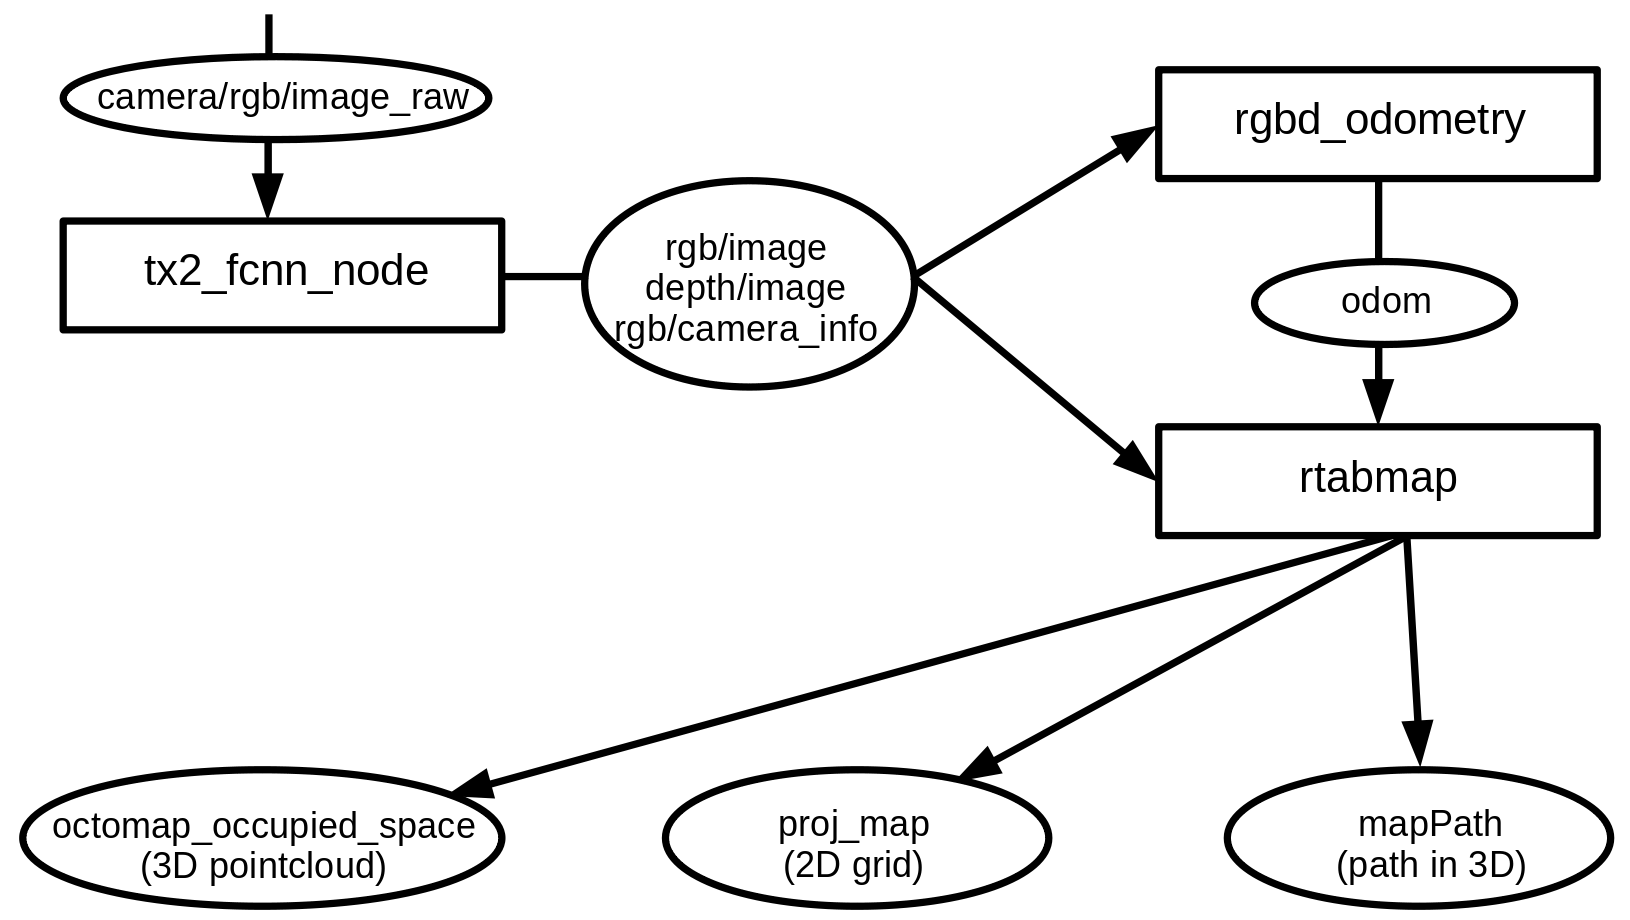
\includegraphics[width=0.7\textwidth]{img/rosnode_scheme.png}
		\caption{Схема ROS-узлов представленного алгоритма vSLAM}
		\label{figure_rosnode}
	\end{figure}
	
	Для взаимодействия нейросети восстановления глубины с алгоритмом RTAB-MAP, а также для облегчения запуска на робототехнической системе была использована библиотека Robot Operating System (ROS)\cite{koubaa2017robot}. Исходный код модуля восстановления глубины в формате ROS-узла, а также инструкции по установке и запуску доступны в репозитории\footnote{https://github.com/cnndepth/tx2\_fcnn\_node}. Схема ROS-узлов разработанного алгоритма vSLAM представлена на рисунке \ref{figure_rosnode}.
	
	\begin{figure}
		\centering
		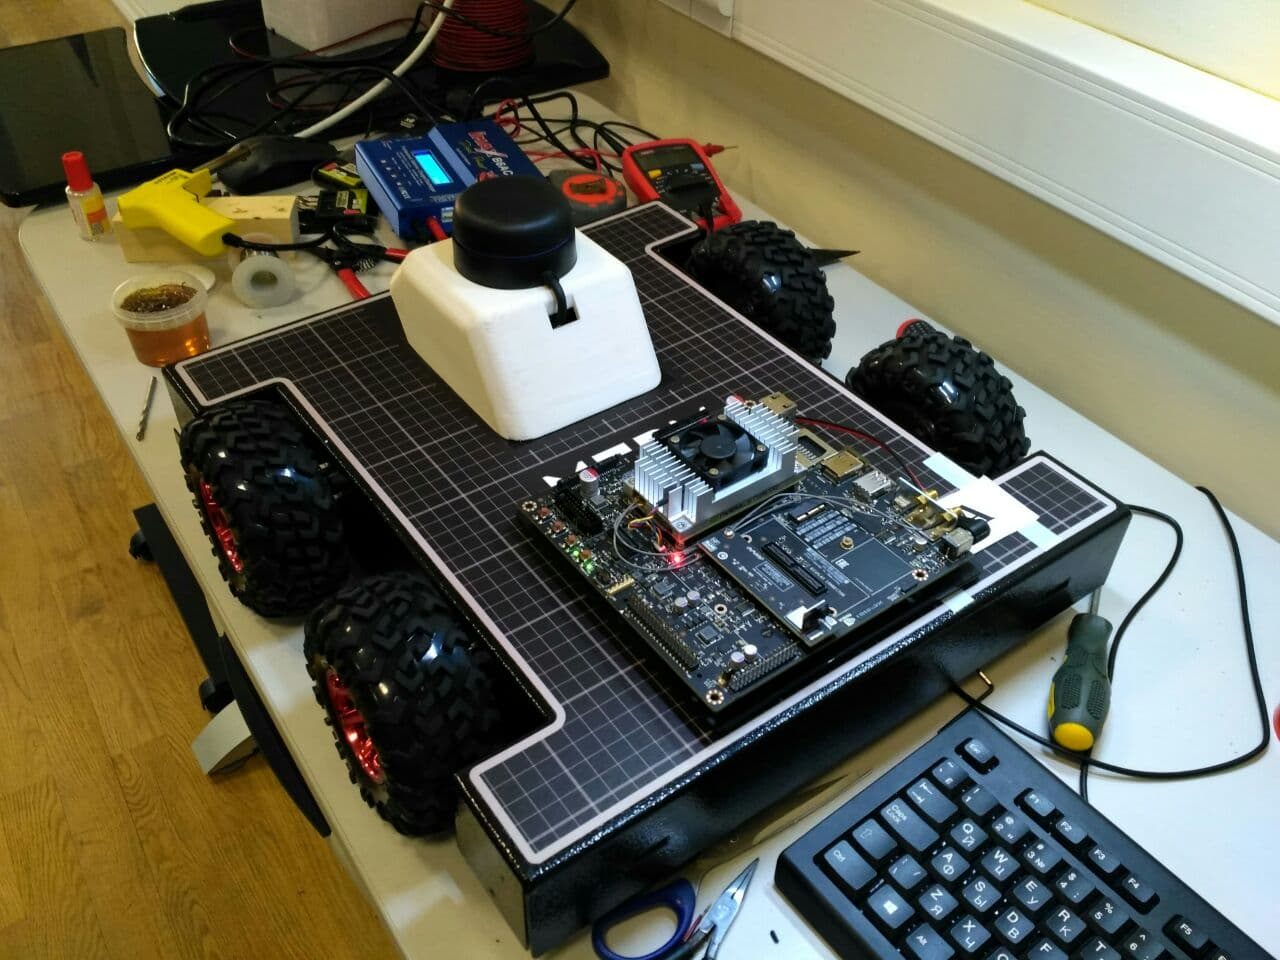
\includegraphics[width=0.3\textwidth]{img/mprm.jpg}
		\caption{Роботехническая платформа МПРМ с установленным на ней компьютером NVidia Jetson TX2}
		\label{figure_mprm}
	\end{figure}
	
	Для оценки качества, эффективности и стабильности разработанного алгоритма vSLAM было проведено два вида экспериментов - в симуляционной среде и на реальном роботе. Для симуляционных экспериментов использовался компьютер со следующими характеристиками:
	
	\begin{itemize}
		\item Процессор: Intel Core i5-9600K, 6 ядер
		\item Видеокарта: GeForce RTX 2060, 1920 CUDA-ядер
		\item Оперативная память: 32 Гб
		\item Видеопамять: 6 Гб
		\item ОС: Ubuntu 18.04
 	\end{itemize}
 
 	В качестве реального робота использовалась колесная платформа МПРМ (см. рис. \ref{figure_mprm}) с установленным на борту компьютером NVidia Jetson TX2 со следующими характеристиками:
 	
 	\begin{itemize}
 		\item Процессор: ARM Cortex, 4 ядра + NVidia Denver, 2 ядра
 		\item Видеокарта: NVidia Pascal GPU, 256 CUDA-ядер
 		\item Оперативная память: 8 Гб
 		\item Видеопамять: общая с оперативной памятью
 		\item ОС: Ubuntu 18.04
 	\end{itemize}
 
 	Подробное описание экспериментов в симуляции и на реальном роботе предоставлено ниже.
	
	\section{Эксперименты}
	
	\subsection{Эксперименты в симуляторе}
	\label{section_experiments}
	
	\begin{table}
		\centering
		\begin{tabular}{|l|c|c|c|c|c|c|}
			\textbf{sample} & \textbf{ATE} & \textbf{AME} & \textbf{AME ours} & \textbf{sATE} & \textbf{sAME} & \textbf{sOAME} \\
			\hline
			1\_first & 3.193 & 0.449 & 3.517 & 0.568 & 0.277 & nan \\
			1\_second & 2.482 & 0.396 & 3.119 & 0.122 & 0.298 & nan \\
			2\_first & 2.31 & 0.414 & 3.065 & 0.679 & 0.259 & nan \\
			2\_second & 2.855 & 0.47 & 3.567 & 0.221 & 0.179 & nan \\
			3\_first & 1.294 & 0.364 & 1.885 & 0.233 & 0.148 & nan \\
			3\_second & 1.042 & 0.415 & 1.589 & 0.224 & 0.252 & nan \\
			4\_first & 2.068 & 0.688 & 3.074 & 0.356 & 0.226 & nan \\
			4\_second & 2.441 & 0.474 & 2.997 & 0.691 & 0.246 & nan \\
			5\_first & 2.94 & 0.329 & 3.281 & 0.338 & 0.186 & nan \\
			5\_second & 1.598 & 0.371 & 1.938 & 0.146 & 0.261 & nan \\
			6\_first & 1.907 & 0.359 & 2.564 & 0.285 & 0.264 & nan \\
			6\_second & 2.766 & 0.362 & 3.438 & 0.256 & 0.197 & nan \\
			7\_first & 0.461 & 0.381 & 1.194 & 0.089 & 0.374 & nan \\
			7\_second & 0.976 & 0.373 & 1.358 & 0.29 & 0.219 & nan \\
			8\_first & 1.462 & 0.4 & 2.2 & 0.16 & 0.192 & nan \\
			8\_second & 0.877 & 0.473 & 1.607 & 0.162 & 0.228 & nan \\
			9\_first & 1.459 & 0.321 & 1.627 & 0.296 & 0.432 & nan \\
			9\_second & 0.162 & 0.174 & 0.438 & 0.162 & 0.174 & nan \\
			10\_first & 1.072 & 0.281 & 1.342 & 0.182 & 0.188 & nan \\
			10\_second & 0.908 & 0.307 & 1.395 & 0.461 & 0.426 & nan \\
			11\_first & 1.331 & 0.292 & 2.06 & 1.027 & 0.402 & nan \\
			11\_second & 2.74 & 0.314 & 3.212 & 0.367 & 0.26 & nan \\
			12\_first & 3.602 & 0.444 & 4.315 & 0.315 & 0.205 & nan \\
			12\_second & 2.479 & 0.633 & 3.457 & 0.237 & 0.274 & nan \\
			13\_first & 3.114 & 0.702 & 3.568 & 0.421 & 0.178 & nan \\
			13\_second & 2.633 & 0.305 & 3.03 & 0.504 & 0.242 & nan \\
			14\_first & 1.843 & 0.304 & 2.643 & 0.182 & 0.208 & nan \\
			14\_second & 1.418 & 0.543 & 2.093 & 0.318 & 0.155 & nan \\
			15\_first & 1.369 & 0.473 & 2.01 & 0.221 & 0.211 & nan \\
			15\_second & 0.688 & 0.314 & 0.952 & 0.356 & 0.274 & nan \\
			16\_first & 2.128 & 0.403 & 2.701 & 0.26 & 0.219 & nan \\
			16\_second & 2.265 & 0.447 & 2.719 & 0.442 & 0.243 & nan \\
			17\_first & 1.054 & 0.336 & 1.503 & 0.203 & 0.157 & nan \\
			17\_second & 0.525 & 0.273 & 1.061 & 0.061 & 0.19 & nan \\
			18\_first & 0.768 & 0.281 & 1.215 & 0.214 & 0.172 & nan \\
			18\_second & 0.991 & 0.316 & 1.395 & 0.375 & 0.356 & nan \\
			19\_first & 0.612 & 0.356 & 1.362 & 0.218 & 0.239 & nan \\
			19\_second & 0.711 & 0.326 & 1.095 & 0.219 & 0.564 & nan \\
			20\_first & 1.672 & 0.297 & 2.021 & 0.23 & 0.208 & nan \\
			20\_second & 1.094 & 0.365 & 1.637 & 0.287 & 0.247 & nan \\
			\hline
			\textbf{Average} & \textbf{1.683} & \textbf{0.388} & \textbf{2.231} & \textbf{0.309} & \textbf{0.251} & \textbf{nan} \\                      
		\end{tabular}
		\caption{Результаты экспериментов с алгоритмом vSLAM на симуляционных данных. ATE, AME, AME ours - значения соответствующих метрик на исходных данных. sATE, sAME, sOAME - значения метрик ATE, AME standard, AME ours после коррекции масштаба}
		\label{table_maomaps_results}
	\end{table}
	
	Для оценки качества предложенного алгоритма vSLAM было проведено масштабное экспериментальное исследование в симуляторе Habitat \cite{savva2019habitat} на датасете из работы \cite{bokovoy2021maomaps}. На каждой из 40 видеопоследовательностей датасета был запущен vSLAM в режиме реального времени. Построенные vSLAM карты и траектории затем сравнивались с истинными для оценки качества. Оценка качества производилась по метрике ATE \ref{eq_ate}, а также по метрике AME \ref{eq_ame} с сопоставлением точек по методу ближайшего соседа (AME) и по ракурсам, как описано в разделе \ref{section_our_ame} (AME ours). Значения метрик приведены в таблице \ref{table_maomaps_results}.
	
	\begin{figure}
		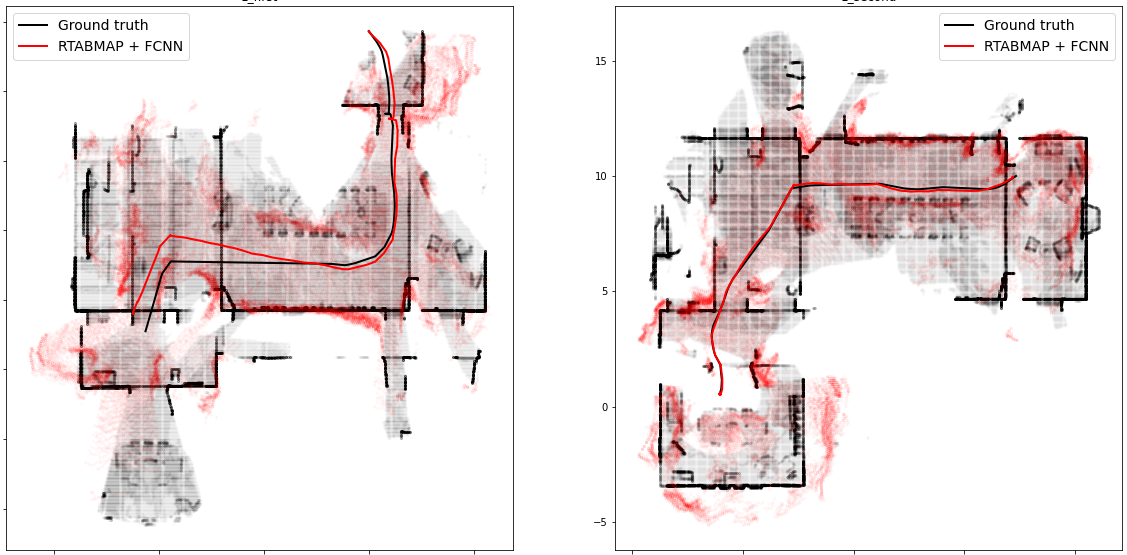
\includegraphics[width=1.0\textwidth]{img/1.png}
		\caption{Примеры карт, построенных методом vSLAM с нейросетевым восстановлением глубины. Черным показаны истинная карта и траектория, красным - восстановленная методом vSLAM}
		\label{figure_slam_map_example}
	\end{figure}
	
	В результате экспериментов выяснилось, что представленный алгоритм vSLAM способен строить правдоподобную карту помещений. Средняя ошибка траектории составила 1.28м, а средняя ошибка картирования - 0.38м по метрике AME standard и 1.76м по метрике AME ours. Такие большие значения ошибки получились из-за некорректного определения масштаба, что связано с различием в параметрах камеры, с которой записана обучающая выборка, и камеры в симуляторе. После коррекции масштаба ошибка уменьшилась примерно в 3 раза по всем метрикам. Примеры карт и траекторий, построенных методом vSLAM, показаны на рисунке \ref{figure_slam_map_example}.
	
	\textbf{TODO:} Добавить метрики после коррекции масштаба!
	
	\subsection{Эксперименты на реальном роботе}
	
	Помимо экспериментов в симуляционной среде, было также проведено тестирование разработанного алгоритма vSLAM в реальном времени на колесной робототехнической платформе МПРМ с бортовым компьютером NVidia Jetson TX2. Восстановление глубины входящих изображений с помощью нейросети производилось на графическом процессоре бортового компьютера, а алгоритм RTAB-MAP выполнялся на центральном процессоре. Таким образом, модули восстановления глубины и картирования работали параллельно, не отнимая ресурсы друг друга.
	
	Эксперимент проводился на полигоне робототехнического центра ФИЦ ИУ РАН. Робот двигался по замкнутой траектории длиной около 40м. Управление движением робота осуществлялось дистанционно через контроллер Raspberry Pi.
	
	По итогам эксперимента, с помощью предложенного алгоритма vSLAM удалось построить правдоподобную карту той части полигона, по которой двигался робот. В начале траектории произошла ошибка определения угла поворота, однако в конце траектории, при успешном замыкании цикла в методе RTAB-MAP, данная ошибка была устранена. Видео с демонстрацией эксперимента доступно по ссылке\footnote{https://drive.google.com/file/d/1eTrlA7D91SNjfQrG0LbKaEpmi511zcAh/view}.
	
	\section{Выводы}
	
	В данной работе был предложен метод одновременного картирования и локализации по данным с единственной видеокамеры, основанный на восстановлении глубин изображений с помощью нейросети и алгоритме RTAB-MAP. Для оценки качества и эффективности предложенного метода были проведены эксперименты в симуляционной среде и на реальном роботе. Эксперименты показали, что данный метод способен работать в реальном времени в условиях ограниченных вычислительных ресурсов и строить плотную трехмерную правдоподобную карту при движении внутри помещения. Высокие значения ошибки на данных из симулятора обусловлены главным образом некорректным определением масштаба, что может быть скорректировано путем изменения обучающей выборки для нейронной сети.
	
	%--------------------------------------------------------------------------------------------------------------------------
	% EXPLORATION
	%--------------------------------------------------------------------------------------------------------------------------
	
	\chapter{Применение в задаче исследования неизвестной местности}
	
	\section{Описание задачи исследования неизвестной местности}
	
	\subsection{Постановка задачи}
	
	Рассматриваемая проблема исследования неизвестной местности (ИНМ) описывается следующим образом. Робот, оснащенный только визуальными датчиками (монокулярная, стерео или RGB-D камера), находится в неизвестной среде ограниченной площади (обычно в закрытом помещении). Его задача - построить двумерную карту окружающей среды, перемещаясь по ней.
	
	\begin{figure}
		\centering
		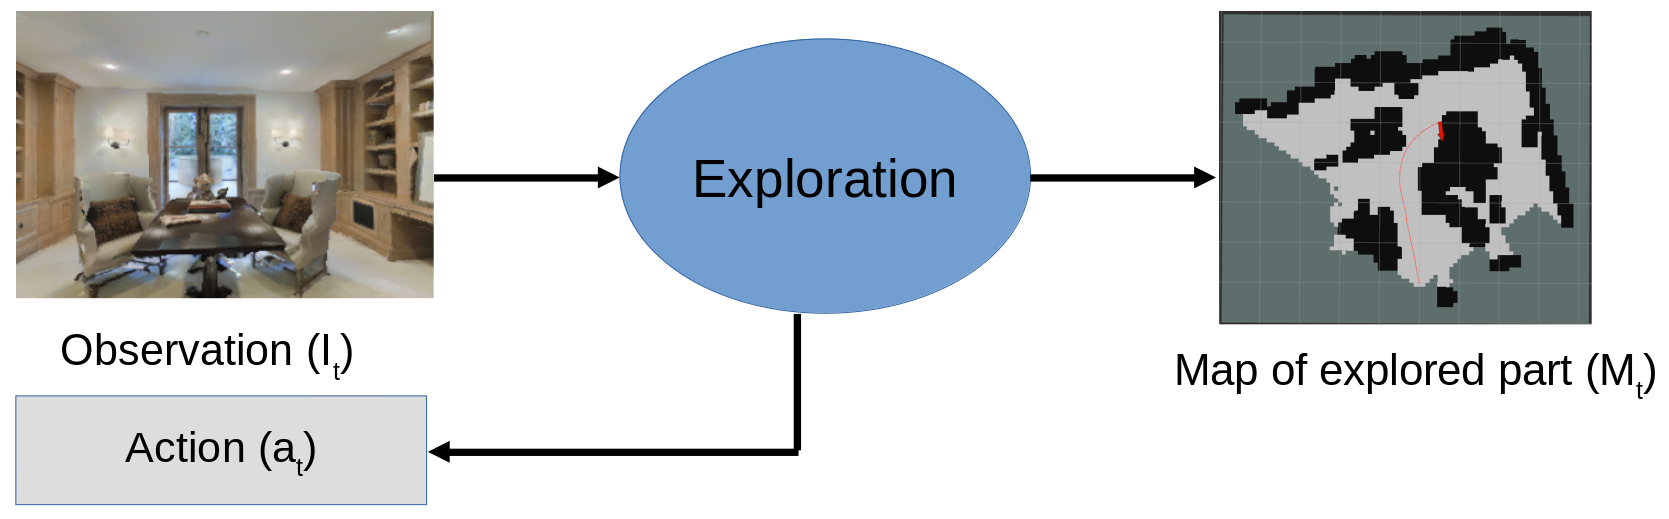
\includegraphics[width=0.9\textwidth]{img/exploration_problem_setting.png}
		\caption{Постановка задачи исследования неизвестной местности}
		\label{figure_exploration_setting}
	\end{figure}
	
	На каждом шаге $ t $ робот получает наблюдение $ I_t $ - изображение с его камеры. Используя это наблюдение, алгоритм ИНМ отслеживает его местоположение, картирует информацию, полученную в результате наблюдения, и решает, куда двигаться, чтобы исследовать и нанести на карту новое пространство. Результатом работы алгоритма $ A $ на шаге $ t $ является $ M_t $ - карта исследованной части окружения и действие $ a_t $ - намерение двигаться в неком направлении (см. рис. \ref{figure_exploration_setting}):
	
	$$ A (I_t, M_ {t-1}) = (M_t, a_t) $$
	
	Карта представлена в виде 2D-матрицы и состоит из свободных, занятых и неисследованных ячеек. Каждая ячейка этой матрицы представляет собой небольшой квадрат фиксированного размера (например, 5x5 см). В карте также указывается положение верхнего левого угла матрицы в глобальной системе координат. На начальном этапе карта представляет собой пустую матрицу.
	
	$$ M_t = (P_t \in \{0, 1, -1 \} ^ {H \times W}; (x_t, y_t) \in \mathbb {R} ^ 2); \ \ M_0 = (\emptyset; (0, 0)) $$
	
	Здесь $0$ кодирует свободную ячейку карты, $1$ - занятую, $-1$ - неисследованную.
	
	Действие представлено в виде изменения позиции робота:
	
	$$ a_t = (dx, dy, \delta) $$
	
	Это команда для робота «двигаться на расстояние $ (dx, dy) $ (относительно его текущего положения) и вращаться на угол $ \delta $». Чтобы упростить нашу модель, мы рассматриваем только четыре возможных действия: двигаться вперед ($ a_t = (dx, 0, 0) $), повернуть налево ($ a_t = (0, 0, \delta) $), повернуть направо ($ a_t = (0, 0, - \delta) $) и оставаться на месте ($ a_t = (0, 0, 0) $).
	
	\subsection{Метрики качества}
	
	Для измерения эффективности ИНМ обычно используются показатели абсолютного и относительного покрытия. Значение абсолютной метрики - это площадь построенной алгоритмом карты на определенных промежутках времени $ t $. Значение относительной метрики - это доля площади окружающей среды, которая была исследована (нанесена на карту) на определенных промежутках времени $ t $:
	
	\begin{equation}
	C_{abs} = \{|(i,j): M_t^{i,j} \geq 0|\}, t \in T
	\label{eq_cov_abs}
	\end{equation}
	
	\begin{equation}
	C_{rel} = \lbrace \frac{|(i,j): M_t^{i,j} \geq 0|}{|(i,j): M^{i,j} \geq 0|} \rbrace, t \in T
	\label{eq_cov_rel}
	\end{equation}
	
	где $M$ - истинная карта окружающей среды.
	
	\section{Описание метода}
	
	\begin{figure}
		\centering
		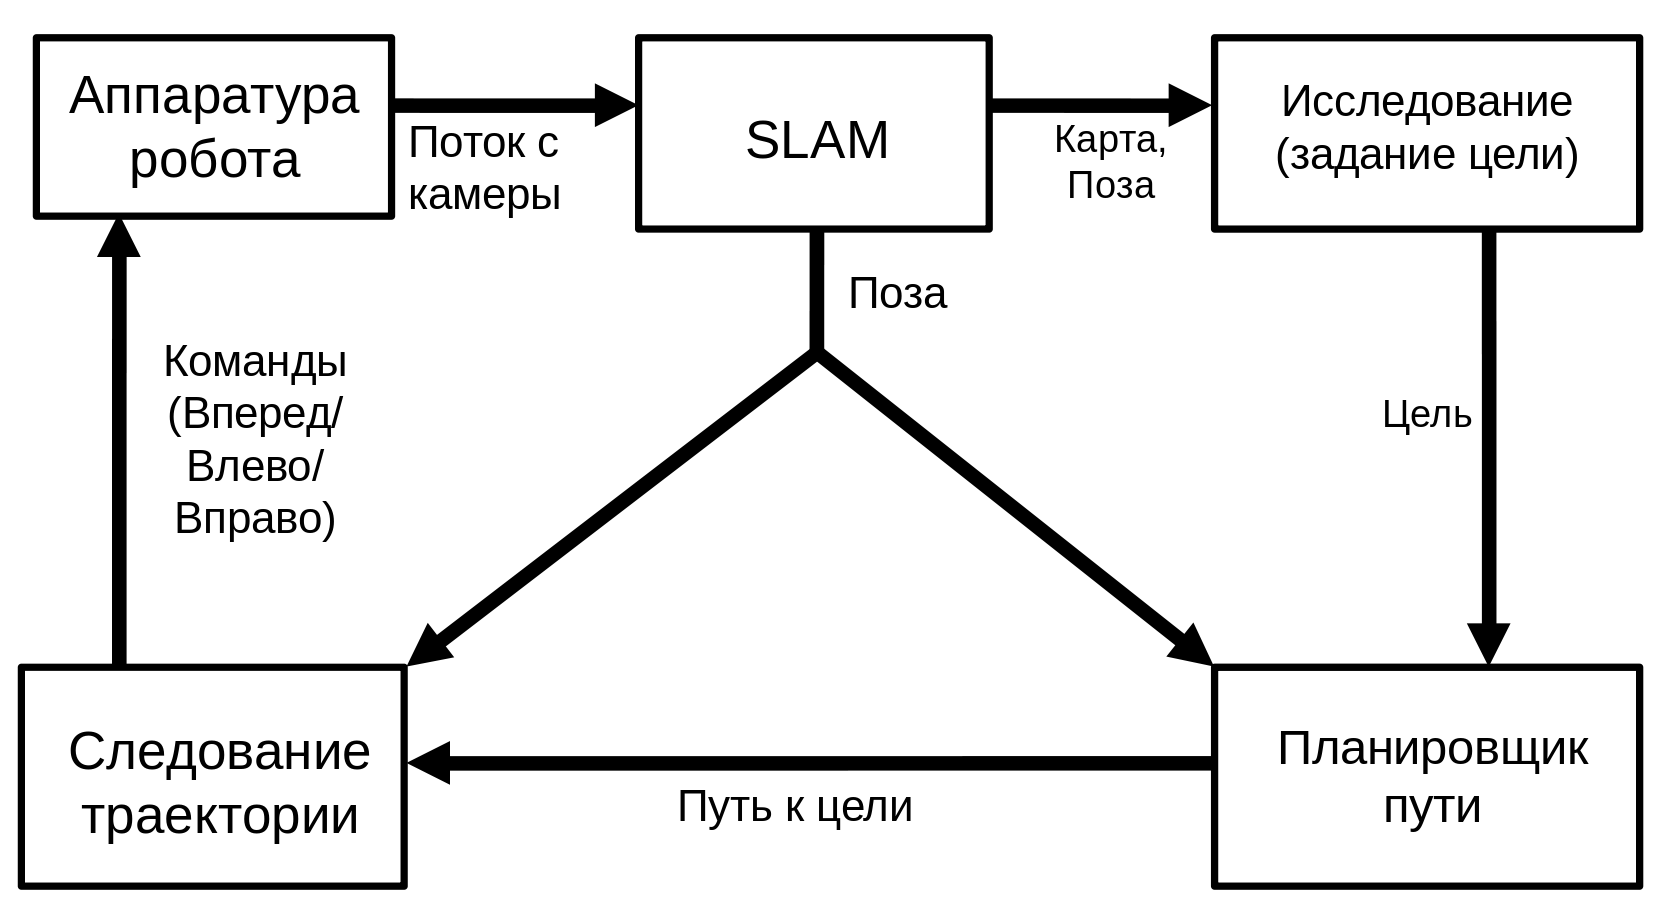
\includegraphics[width=0.8\textwidth]{img/pipeline_scheme_rus.png}
		\caption{Схема организации работы алгоритма автономной навигации}
		\label{figure_pipeline}
	\end{figure}
	
	В работе предложен алгоритм для полностью автономного исследования неизвестной местости с помощью vSLAM. Алгоритм состоит из следующих шагов: 
	
	\begin{itemize}
		\item Модуль \textbf{одновременного картирования и локализации (SLAM)} получает данные с камеры робота и оценивает его вычисляет траекторию и 2D-карту окружающей среды в реальном времени 
		\item Модуль \textbf{исследования неизвестной местности (ИНМ)} берет текущее положение робота и построенную модулем SLAM карту, и выбирает целевую точку, к которой должен идти робот 
		\item Модуль \textbf{планирования пути} строит путь от робота до позиции цели на созданной SLAM карте 
		\item Модуль \textbf{следования по траектории} принимает текущее положение робота и путь к цели и задает низкоуровневые команды контроллеру робота - куда двигаться: вперед, влево или вправо 
	\end{itemize}

	\begin{figure}
		\centering
		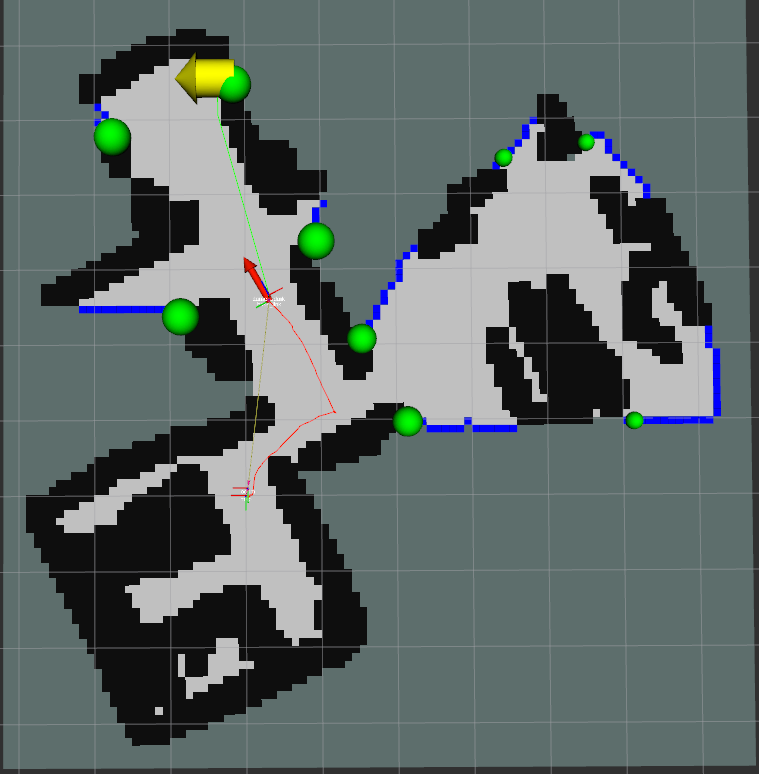
\includegraphics[width=0.4\textwidth]{img/exploration_sample.png}
		\caption{Пример работы ИНМ, основанного на поиске границ. Черная область - это занятые ячейки карты, белая область - свободные ячейки карты, синие линии - границы, красная стрелка - позиция робота, а большая желтая стрелка - цель, выбранная алгоритмом. Зеленые круги отображают стоимость границ - чем больше круг, тем ценнее граница. }
		\label{figure_frontiers}
	\end{figure}
	
	С целью упрощения реализации на роботе и взаимодействия между модулями предложенный алгоритм был разработан с использванием программной библиотеки Robot Operaing System (ROS)\footnote {http://www.ros.org}. Полная схема взаимодействия модулей представлена на рисунке \ref{figure_pipeline}.
	
	Подробное описание модуля SLAM приведено в предыдущей главе. Для постановки целей используется алгоритм, основанный на ROS-пакете \texttt{explore\_lite} \footnote{http://wiki.ros.org/explore\_lite}, описанный в работе ~\cite{Horner2016}. Алгоритм постановки целей ищет границы между свободным и неизвестным пространством на карте, построенной в 2D SLAM. Чтобы найти эти границы, используется поиск в ширину (BFS) в графе. После выполнения поиска вычисляется стоимость всех границ исходя из расстояния до них и их размера. Центроид наиболее ``ценной'' границы помечается как цель для робота. Пример границ и цели показан на рисунке \ref{figure_frontiers}.
	
	В данной работе в базовый алгоритм постановки целей из пакета \texttt{explore\_lite} были внесены некоторые улучшения для повышения его эффективности и стабильности. В частности, была изменена функция стоимости границ - расстояния до границ вычисляются как длины пути в построенной модулем SLAM карте, также учитывается ориентация робота и направление от его позиции до границы. Помимо этого, было добавлено расширение препятствий в построенной модулем SLAM карте, что позволило алгоритму ИНМ находить меньше некорректных путей и работать более стабильно. Также, во избежание застревания перед невидимым препятствием, был добавлен ``детектор столкновений'', который срабатывает, когда модуль следования траектории дает команду ``вперед'', а модуль SLAM фиксирует отсутствие движения робота.
	
	\begin{figure}
		\centering
		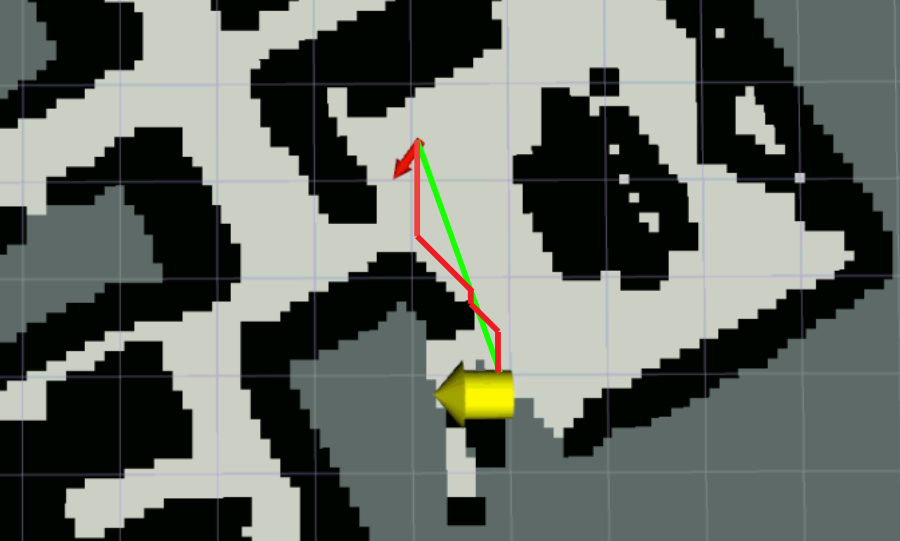
\includegraphics[width=0.5\textwidth]{img/paths_truncated.png}
		\caption{Пример пути, построенного алгоритмами A* (красный) и Theta* (зеленый) }
		\label{figure_thetastar_path}
	\end{figure}
	
	Для планирования пути от робота к цели был использован алгоритм Theta*~\cite{nash2007theta}. Этот алгоритм имеет высокую вычислительную эффективность и строит пути с произвольным углом. Таким образом, пути, построенные Theta* в двумерной карте короче и намного плавнее, чем пути традиционных алгоритмов, таких как алгоритм Дейкстры~\cite{dijkstra1959note} или A*~\cite{hart1968formal} (см. Рис. \ref{figure_thetastar_path}). Плавность траектории критически важна для систем визуального картирования и локализации, поскольку резкие движения могут сделать vSLAM нестабильным.
	
	Для перемещения робота по предложенному пути используется простой и понятный алгоритм. Ориентация робота сравнивается с направленим от позиции робота до следующей точки пути. Если угол между ориентацией робота и направлением на точку пути ниже некоторого порогового значения (например, менее 5 градусов по модулю), робот перемещается вперед. Если он выше порога и отрицателен, поворачиваем робота налево. Если он выше порога и положительный, поворачиваем робота вправо.
	
	\section{Эксперименты}
	
	\begin{figure}
		\centering
		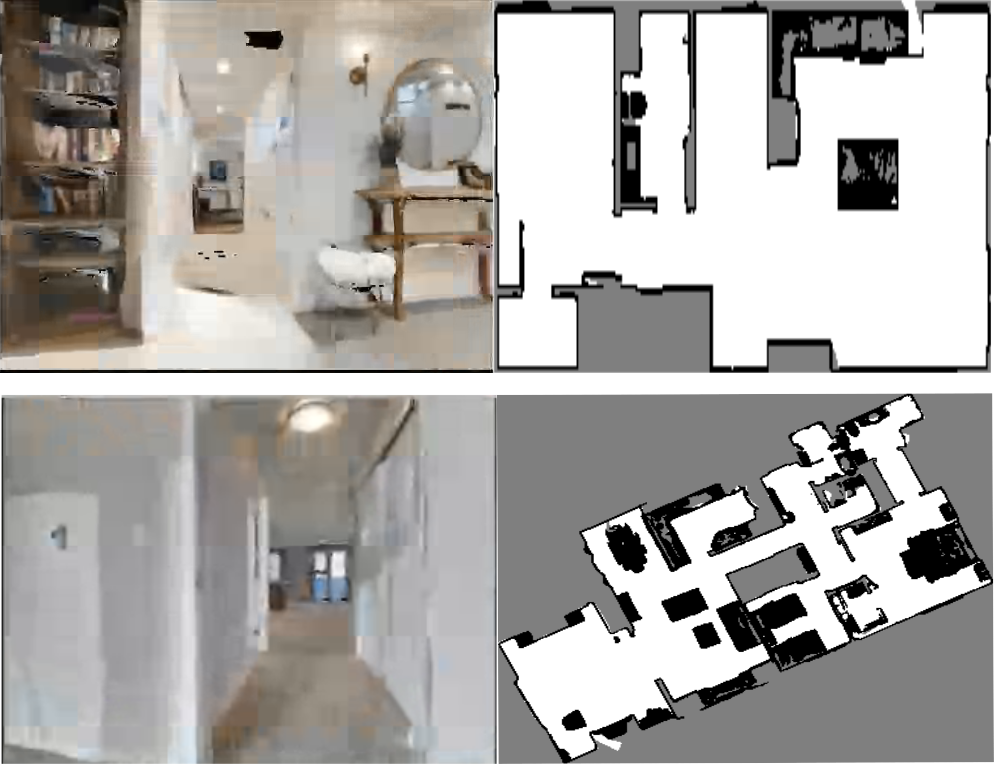
\includegraphics[width=0.7\textwidth]{img/gibson_sample_with_map.png}
		\caption{Изображения и карты некоторых сцен набора данных Gibson}
		\label{figure_gibson_env}
	\end{figure}
	
	Экспериментальное исследование алгоритма ИНМ проводилось на датасете Gibson \cite{xia2018gibson} в симуляторе Habitat \cite{savva2019habitat}. Для экспериментов из 493 сцен датасета была отобрана 31 сцена без лестниц и дефектов текстуры. Площадь выбранных сцен варьировалась от 28 до 251 $\text{м}^2$. Пример изображений и карт этих сцен показан на рис. \ref{figure_gibson_env}.
	
	Для измерения эффективности исследования неизвестной местности была использована метрика покрытия - площадь пространства карты, исследованного в определенный момент времени. Была измерена как абсолютная, так и относительная площадь. Значения площадей измерялись для разного времени, отсчитанного от старта - от 15 до 240 с.
	
	Чтобы исследовать разработанную систему в монокулярном режиме, было проведено несколько экспериментов на выбранных сценах. Для предсказания глубины использовалась полносверточная нейронная сеть, описанная в главе \ref{chapter_our_slam}. Чтобы адаптировать эту нейросеть к симуляционной среде Habitat и параметрам используемой в Habitat камеры, она было дообучена на выборке из порядка 38000 пар изображение-глубина, собранной по 25 сценам выбранной коллекции. Остальные 6 выбранных сцен были использованы для тестирования алгоритма ИНМ.
	
	\begin{figure}
		\centering
		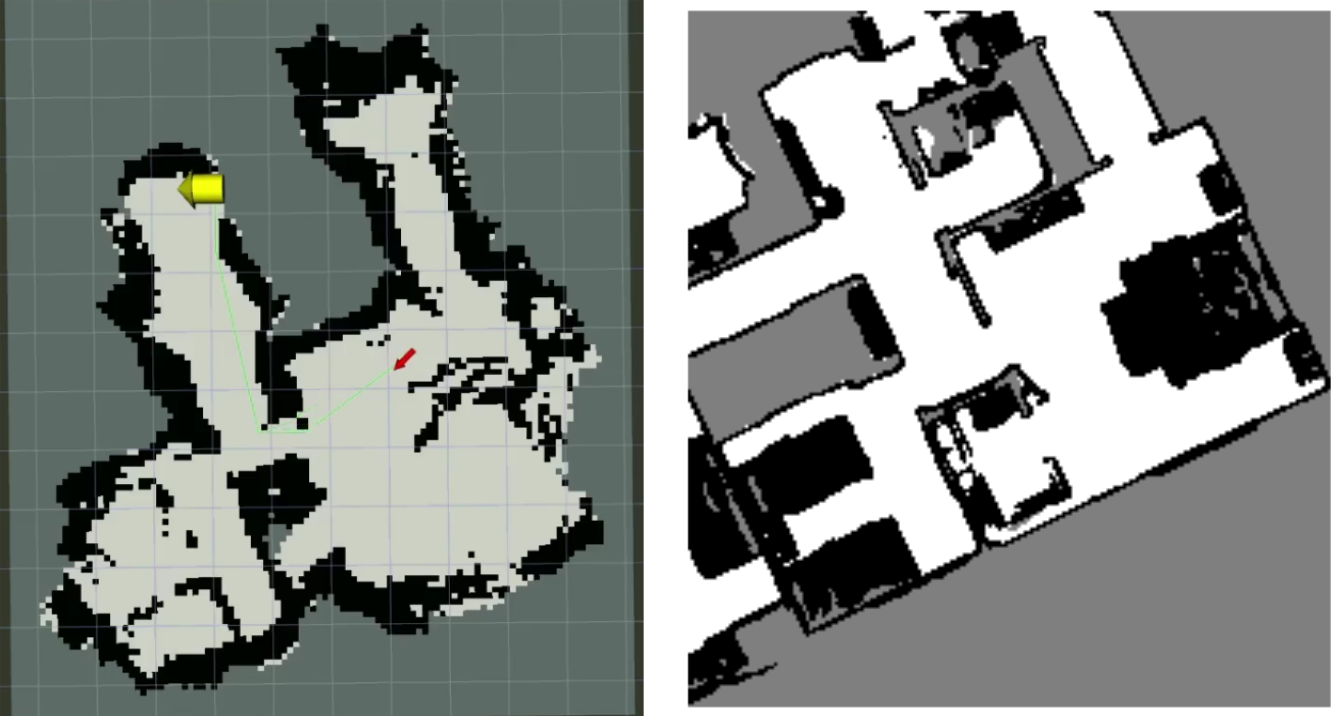
\includegraphics[width=0.8\textwidth]{img/fcnn_map_example.png}
		\caption{Пример карты, построенной при исследовании с глубинами FCNN (слева) по сравнению с истинной картой (справа) }
		\label{figure_fcnn_map_example}
	\end{figure}
	
	\begin{figure}
		\centering
		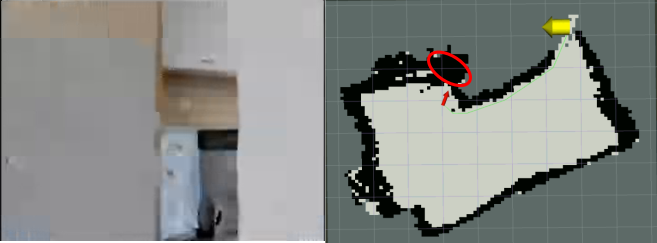
\includegraphics[width=0.7\textwidth]{img/camera_view.png}
		\caption{Пример неточного картирования с предсказанными FCNN глубинами. В поле зрения камеры (левая часть изображения) наблюдается небольшой дверной проем. Но на карте (правая часть рисунка) дверной проем отмечен как стена (см. красный эллипс). }
		\label{figure_doorway_ignore}
	\end{figure}
	
	\begin{figure}
		\centering
		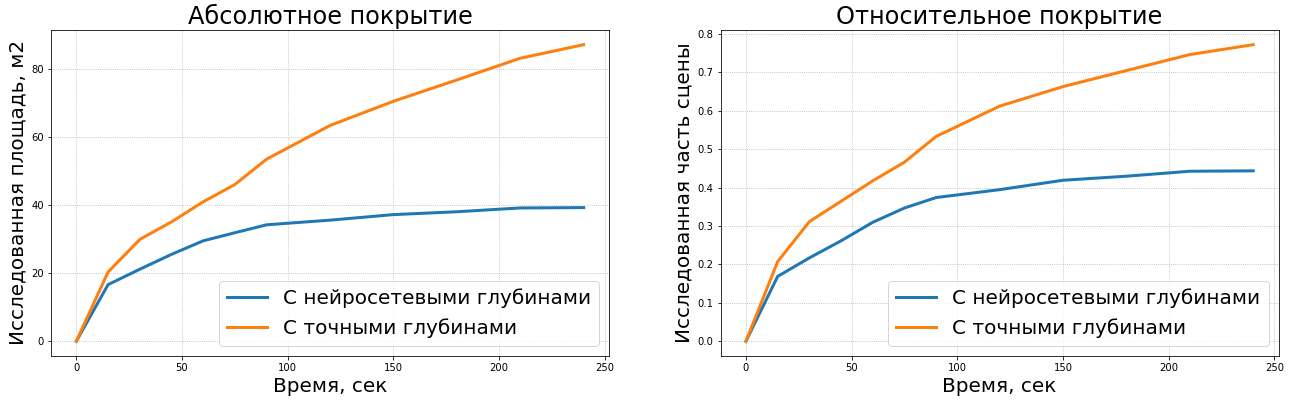
\includegraphics[width=0.9\textwidth]{img/test_fcnn_rus.png}
		\caption{Сравнение работы ИНМ с предсказанными FCNN глубинами и с точными глубинами: абсолютное покрытие (слева) и относительное покрытие сцены (справа) }
		\label{figure_fcnn_metrics}
	\end{figure}
	
	Эксперименты показали, что полученная система может работать автономно и строить правдоподобную карту (см. Рис. \ref{figure_fcnn_map_example}) в монокулярном режиме. Однако ошибки в оценке глубины нейросетью вызвали некоторые отклонения в построенной карте. Например, узкие дверные проемы иногда отображались как сплошная стена (см. Рис.\ref{figure_doorway_ignore}). Из-за такого неточного отображения планировщик не мог найти пути к далеким целям, и алгоритм исследовал только часть сцены. Значения показателей покрытия показаны на рисунке \ref{figure_fcnn_metrics}. Средняя исследованная часть сцены достигла 44 \%.
	
	В целом, тесты показали, что предлагаемая система способна работать в монокулярном режиме с нейросетевым восстановлением глубины, но неточное предсказание глубины может привести к ошибкам при картировании и неполному покрытию сцены. Возникающие ошибки могут быть устранены путем более тщателього обучения нейронной сети и точной настройки параметров SLAM. Видеозапись эксперимента с предлагаемой системой ИНМ доступна по ссылке\footnote{https://drive.google.com/file/d/1QJWmjR9Y2VWbycZVwz3Y6Dl9Rzkp-zjB/view?usp=sharing}.
	
	\section{Выводы}
	
	В данной работе представленный алгоритм vSLAM был интегрирован в систему автономного исследования неизвестной местности. Для оценки качества работы системы было проведено экспериментальное исследование на датасете Gibson в фотореалистичном симуляторе Habitat. В результате экспериментов среднее значение покрытия площади сцены составило 44\% за 240 секунд работы алгоритма. Причиной неполного покрытия сцены являются ошибки картирования, возникающие из-за неточного определения глубины нейросетью. Данные ошибки могут быть устранены путем более тщательного обучения нейросети.
	
	%----------------------------------------------------------------------------------------------------------------------
	% CONCLUSION
	%----------------------------------------------------------------------------------------------------------------------
	
	\chapter{Заключение}
	
	В данной работе был рассмотрен подход к решению задачи одновременного картирования и локализации по видеоданным (vSLAM) в реальном времени в контексте автономной навигации малого мобильного робота в неизвестной местности. Данный подход основан на восстановлении карт глубин изображений с помощью полносверточных нейронных сетей и методе одновременного картирования и локализации RTAB-MAP. Для эффективной работы нейросети в реальном времени в условиях ограниченных вычислительных ресурсов были применены различные архитектурные и технические оптимизации.
	
	Для оценки качества предложенного метода vSLAM была собрана коллекция данных в фотореалистичном симуляторе Habitat, также был использован оригинальный подход к оценке качества построенной алгоритмом vSLAM карты, учитывающий контекст задачи vSLAM. С целью оценки качества предложенного алгоритма vSLAM были проведены эксперименты на собранной коллекции данных, а также на колесной робототехнической платформе с компьютером NVidia Jetson TX2. Эксперименты показали, что предложенный алгоритм способен строить плотную правдоподобную карту местности в реальном времени по данным с единственной видеокамеры.
	
	С целью оценки применимости предложенного метода vSLAM для автономной навигации роботов, данный метод был интегрирован в систему исследования неизвестной местности (ИНМ). Было проведено экспериментальное исследование полученной системы в фотореалистичном симуляторе Habitat. Помимо задачи vSLAM, в ходе экспериментов с помощью системы ИНМ решались задачи постановки целей, а также планирования и следования траектории. Эксперименты показали, что с использованием предложенного метода vSLAM система ИНМ способна функционировать полностью автономно в реальном времени, строить правдоподобные карты помещений и планировать в них маршруты.
	
	Программная реализация предложенного метода vSLAM интегрирована с библиотекой Robotic Operating System (ROS) и выложена в открытый доступ. Исходный код алгоритма, а также параметры запуска, инструкции по установке и утилиты для работы с нейронными сетями доступны в репозитории\footnote{https://github.com/cnndepth/tx2\_fcnn\_node}.
	 
	\printbibliography
\end{document}